\documentclass[runningheads]{llncs}
\usepackage{fullpage}
\usepackage{graphicx} % for including images
\usepackage[T1]{fontenc}
\usepackage{subcaption}
\usepackage{url}
\usepackage{xcolor}
\definecolor{darkred}{rgb}{0.6, 0, 0}
\definecolor{darkgreen}{rgb}{0, 0.5, 0}
\definecolor{darkblue}{rgb}{0, 0, 0.5}
\definecolor{darkmagenta}{rgb}{0.5, 0, 0.5}
\usepackage{hyperref}
\hypersetup{
    colorlinks=true,      % Enable colored links
    linkcolor=darkred,    % Color for internal links
    filecolor=darkgreen,  % Color for file links
    urlcolor=darkblue,    % Color for external URLs
    citecolor=darkmagenta % Color for citations
}


\begin{document}
\title{Enhancing Urban Building Simulations in HiDALGO2 through CI/CD Innovations}
\author{Vincent Chabannes \inst{1}\orcidID{0000-1111-2222-3333} \and
Javier Cladellas \inst{1}\orcidID{} \and 
Abdoulaye Diallo \inst{1}\orcidID{} \and
Maryam Maslek \inst{1}\orcidID{} \and
Philippe Pinçon \inst{1}\orcidID{} \and
Christophe Prud'homme\inst{1}\orcidID{0000-0003-2287-2961}}
\institute{Cemosis, IRMA UMR 7501, University of Strasbourg, CNRS\\ 
\email{\{vincent.chabannes,christophe.prudhomme\}@cemosis.fr}}
\authorrunning{V. Chabannes and C. Prud'homme}


\maketitle

\begin{abstract}
The building sector in the European Union significantly impacts energy consumption and greenhouse gas emissions. The EU's Horizon 2050 initiative sets ambitious goals to reduce these impacts through enhanced building renovation rates. The HiDALGO2 project supports this initiative by developing high-performance computing solutions, specifically through the Urban Building pilot application, which utilizes advanced CI/CD methodologies to streamline simulation and deployment across various computational platforms.
\keywords{HPC, Urban building, City Energy Simulation.}

\end{abstract}

\section{Introduction}
The building sector accounts for approximately 40\% of final energy consumption and 36\% of greenhouse gas emissions within the European Union. In response, the EU has established ambitious targets under the Horizon 2050 framework to double energy renovation rates over the next decade, highlighting the need for innovative solutions to drive these initiatives forward. The HiDALGO2 project, with its focus on high-performance computing and advanced simulations, is at the forefront of tackling this challenge, particularly through its Urban Building pilot application.

The Urban Building pilot in HiDALGO2 aims to leverage high-performance computing to enhance urban simulations for better energy management and air quality assessment. This section outlines the specific objectives and expected impacts of the project.

Advanced simulation tools are employed to predict energy consumption, thermal comfort, and indoor air quality across both the building and urban scales. These simulations support detailed analysis at the individual building level and extend to broader urban environments, influencing urban planning and policy-making.

Integrating building simulations with urban air pollution models enables the project to assess the environmental impact of building stocks comprehensively. This integration improves the predictive accuracy of the simulations by incorporating real-time data such as wind speed and solar radiation, enhancing the models' responsiveness to environmental conditions.

Implementing these objectives will facilitate more informed urban planning decisions, support policy development for energy efficiency, and contribute to reducing urban greenhouse gas emissions. The project also focuses on enhancing the interaction between different environmental models to provide a holistic view of urban ecosystems.

Feel++\cite{christophe_prudhomme_feelppfeelpp_2024}

\section{Current Urban Building Workflow}

\begin{figure}
    \centering
    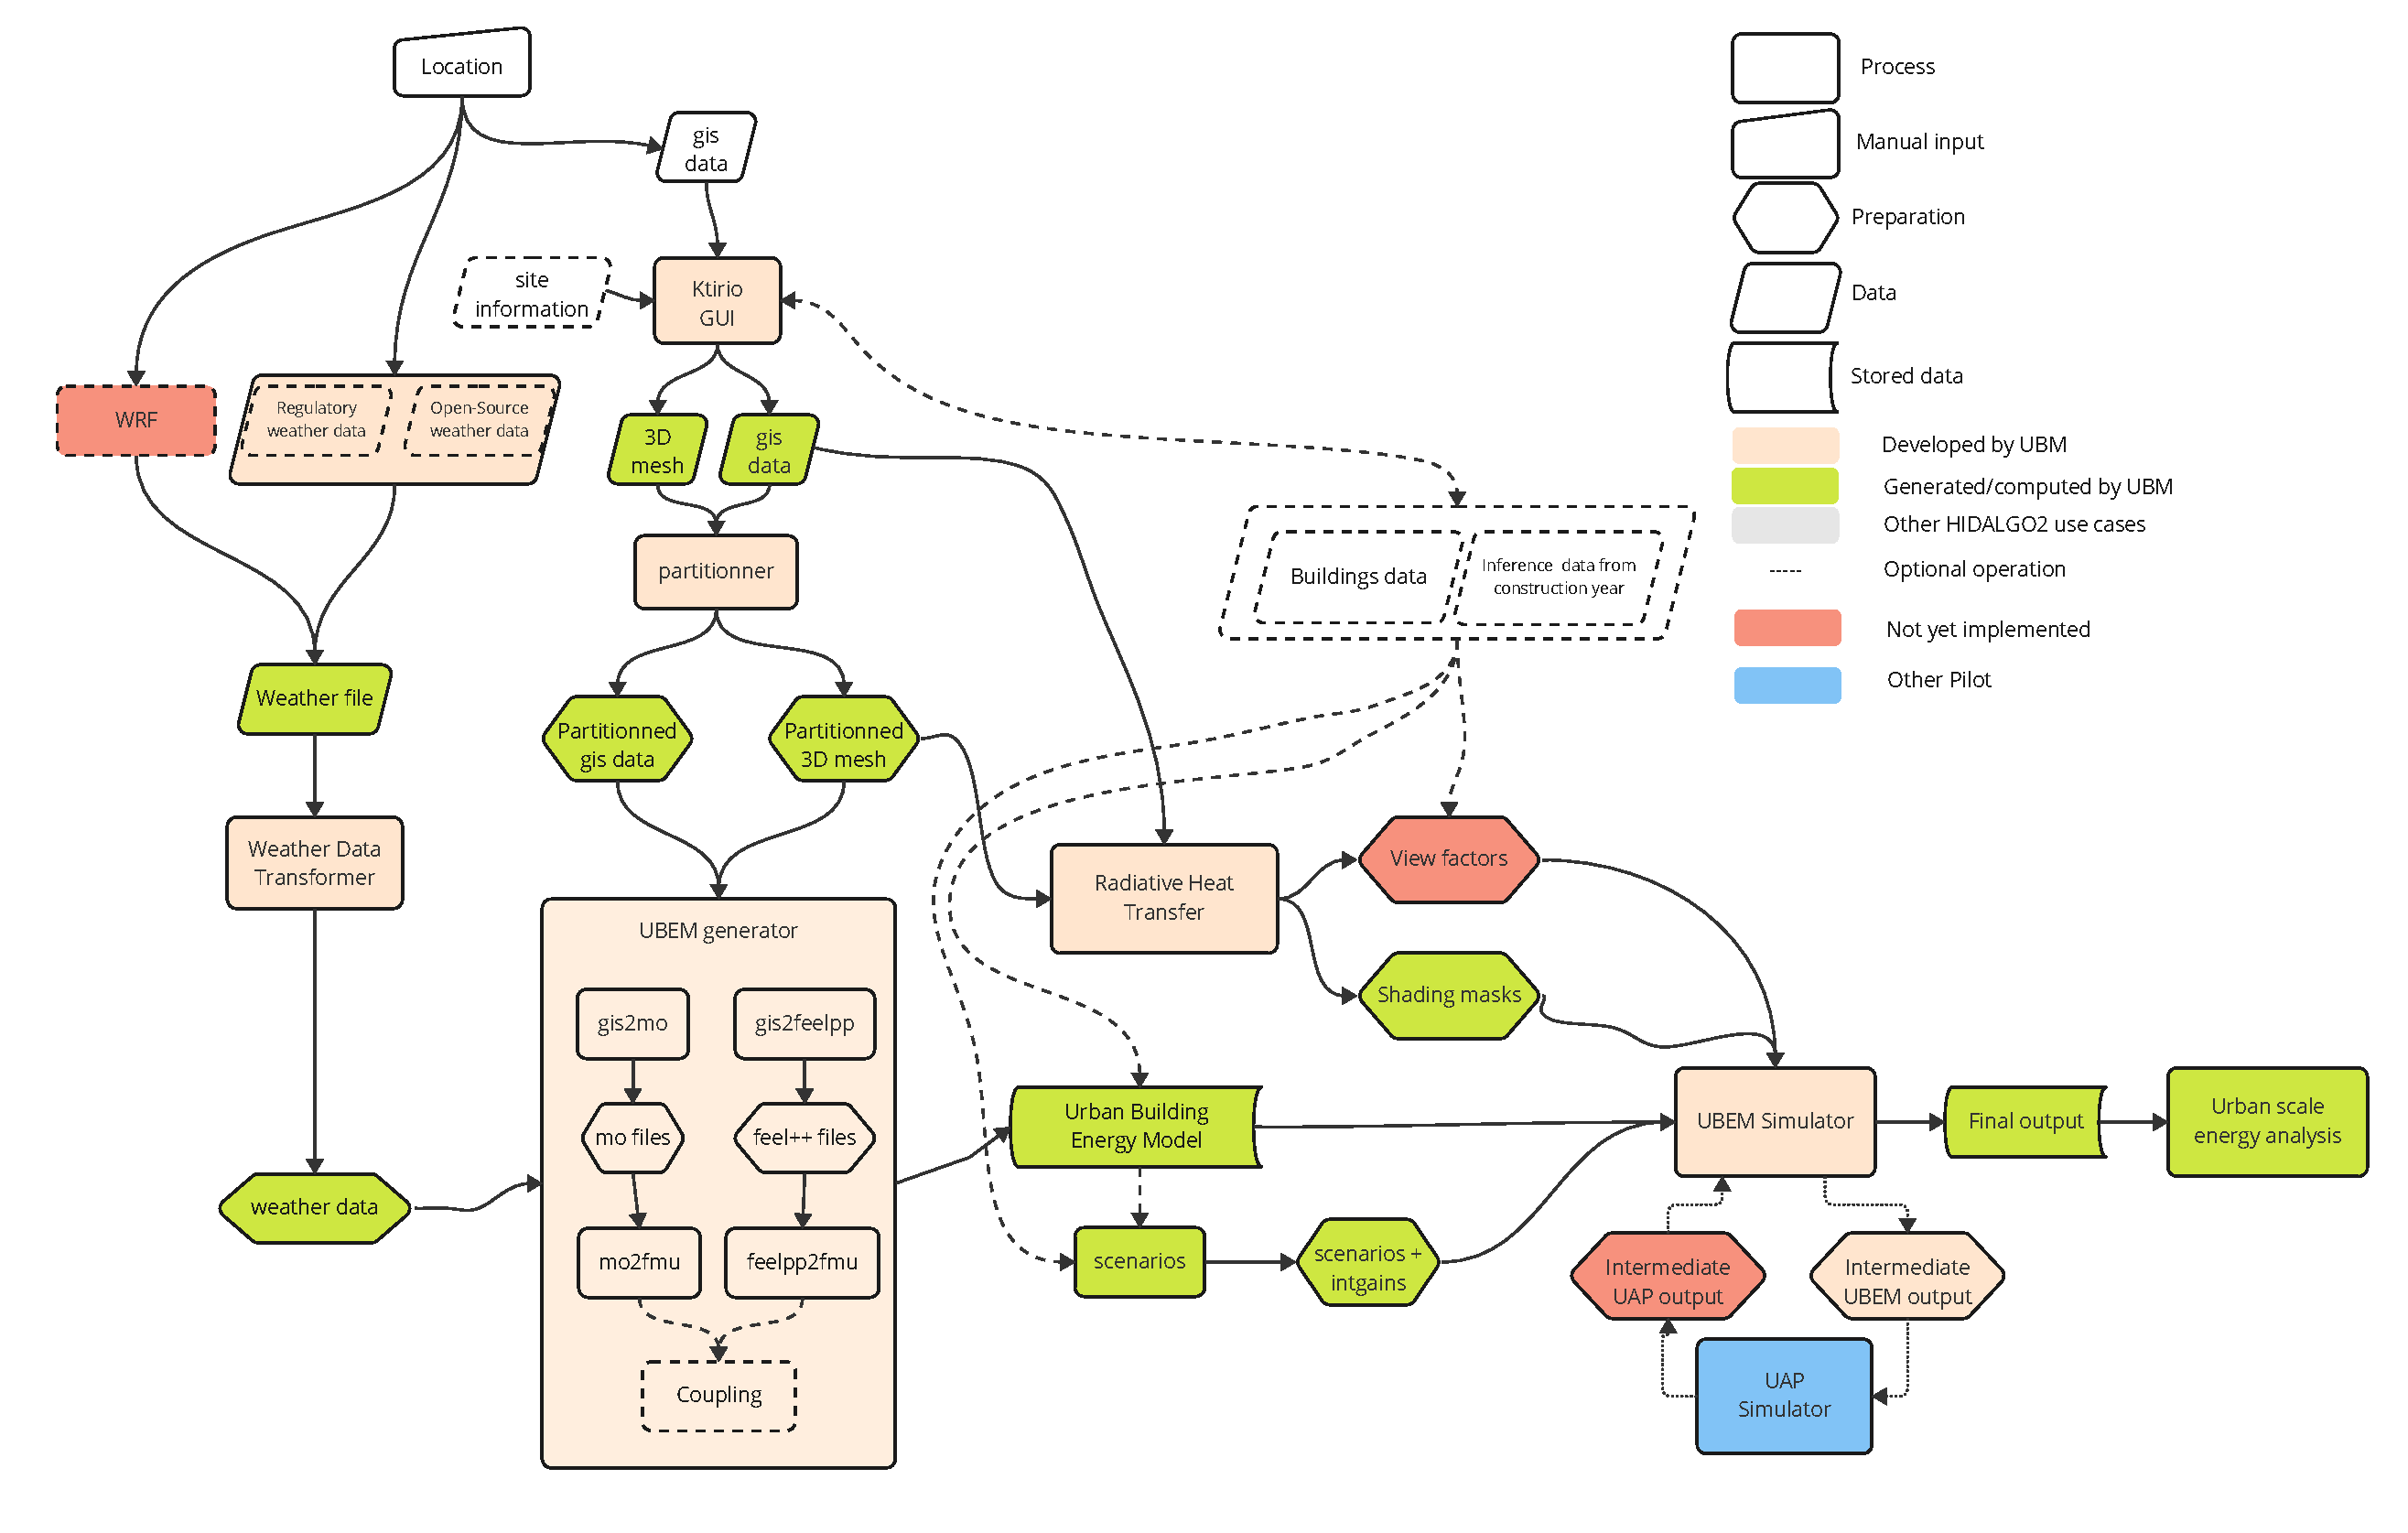
\includegraphics[width=.9\textwidth]{images/kub-workflow.pdf}
    \caption{Current Urban Building Workflow}
    \label{fig:ub_workflow}
\end{figure}

The urban building workflow integrates various data sources and computational tools to effectively simulate and analyze urban building energy and its impact on urban environments. The process encompasses data acquisition, processing, simulation, and analysis, coupled with an integration into urban air pollution models.

\subsection{Data Handling and Simulation Process}
The workflow begins with the collection and preparation of GIS and weather data, transforming it into a format usable for simulations. This data is then partitioned for scalable processing, and converted into Modelica and Feel++ compatible formats through the UBEM Generator.

Using the Urban Building Energy Model (UBEM), this processed data is employed to simulate energy consumption and indoor environmental quality. The simulation focuses on radiative heat transfer, enhancing the accuracy of the energy models. It also computes view factors and shading masks, assessing how buildings affect each other’s exposure to natural light and heat, which influences the urban heat island effect and overall building energy needs.

The building simulation outputs are then fed into the Urban Air Pollution (UAP) simulator to evaluate the impact of building emissions on urban air quality. A feedback loop refines the building simulation scenarios based on intermediate outputs from the UAP simulator, ensuring that the models accurately reflect the complex interdependencies between urban building energy usage and urban air quality.

\subsection{Final Analysis and Urban Scale Energy Evaluation}
The final step involves the UBEM Simulator, which generates outputs summarizing the overall energy consumption and environmental impact of buildings at an urban scale. This comprehensive urban scale analysis merges data from both the building energy models and air quality models to provide a holistic view of urban environmental quality.

This streamlined workflow is critical for accurately simulating and understanding urban sustainability challenges, supporting the broader objectives of our application to improve urban living conditions and environmental impact.


\section{Overview of Urban Building Modeling and Simulation}

We now provide an overview of the geometrical and physical modeling and simulation components of the Urban building application.

\subsection{Geometry Reconstruction of the Urban Model}

The geometric reconstruction of urban environments within the HiDALGO2 project involves a sophisticated approach to creating multi-fidelity representations of buildings, terrain, vegetation, roads, and other urban elements. This section outlines the methodologies employed and the various levels of detail (LOD) used in the models.

The primary challenge lies in accurately representing the complex urban landscape to support various simulations. A tiled web map approach is adopted, which allows for distributed data management and adapts the Level of Definition (LOD) based on specific needs. However, this approach requires the careful integration of tiles to ensure seamless representation.

We describe our definition of Levels of Detail for Buildings
\begin{itemize}
    \item \textbf{LOD-0:} The simplest form, representing buildings as oriented bounding boxes. This level is typically used for large-scale preliminary analyses and quick visual assessments.
    \item \textbf{LOD-1:} Buildings are represented as polygonal extrusions, with added roof structures to improve the visual accuracy and utility in simulations that do not require detailed internal features.
    \item \textbf{LOD-2:} At this level, buildings are detailed using Industry Foundation Classes (IFC) standards, supporting detailed thermal and structural analyses. This includes detailed geometries for each entity of the building, often using complex surface models like B-REP, swept solids, or CSG techniques.
\end{itemize}


In the figure~\ref{fig:buildings}, we illustrate the different levels of details. Panel~\ref{fig:building-lod0} displays the LOD-0 of a building with its bounding box.
Panel~\ref{fig:building-lod1} displays the LOD-1 of a building using its footprint elevated to its height. 
Panel~\ref{fig:building-lod2} and~\ref{fig:building-lod2-zoom} display the LOD-2 representation using BIM.

\begin{figure}[htbp]
\centering
\begin{subfigure}{.4\textwidth}
  \centering
  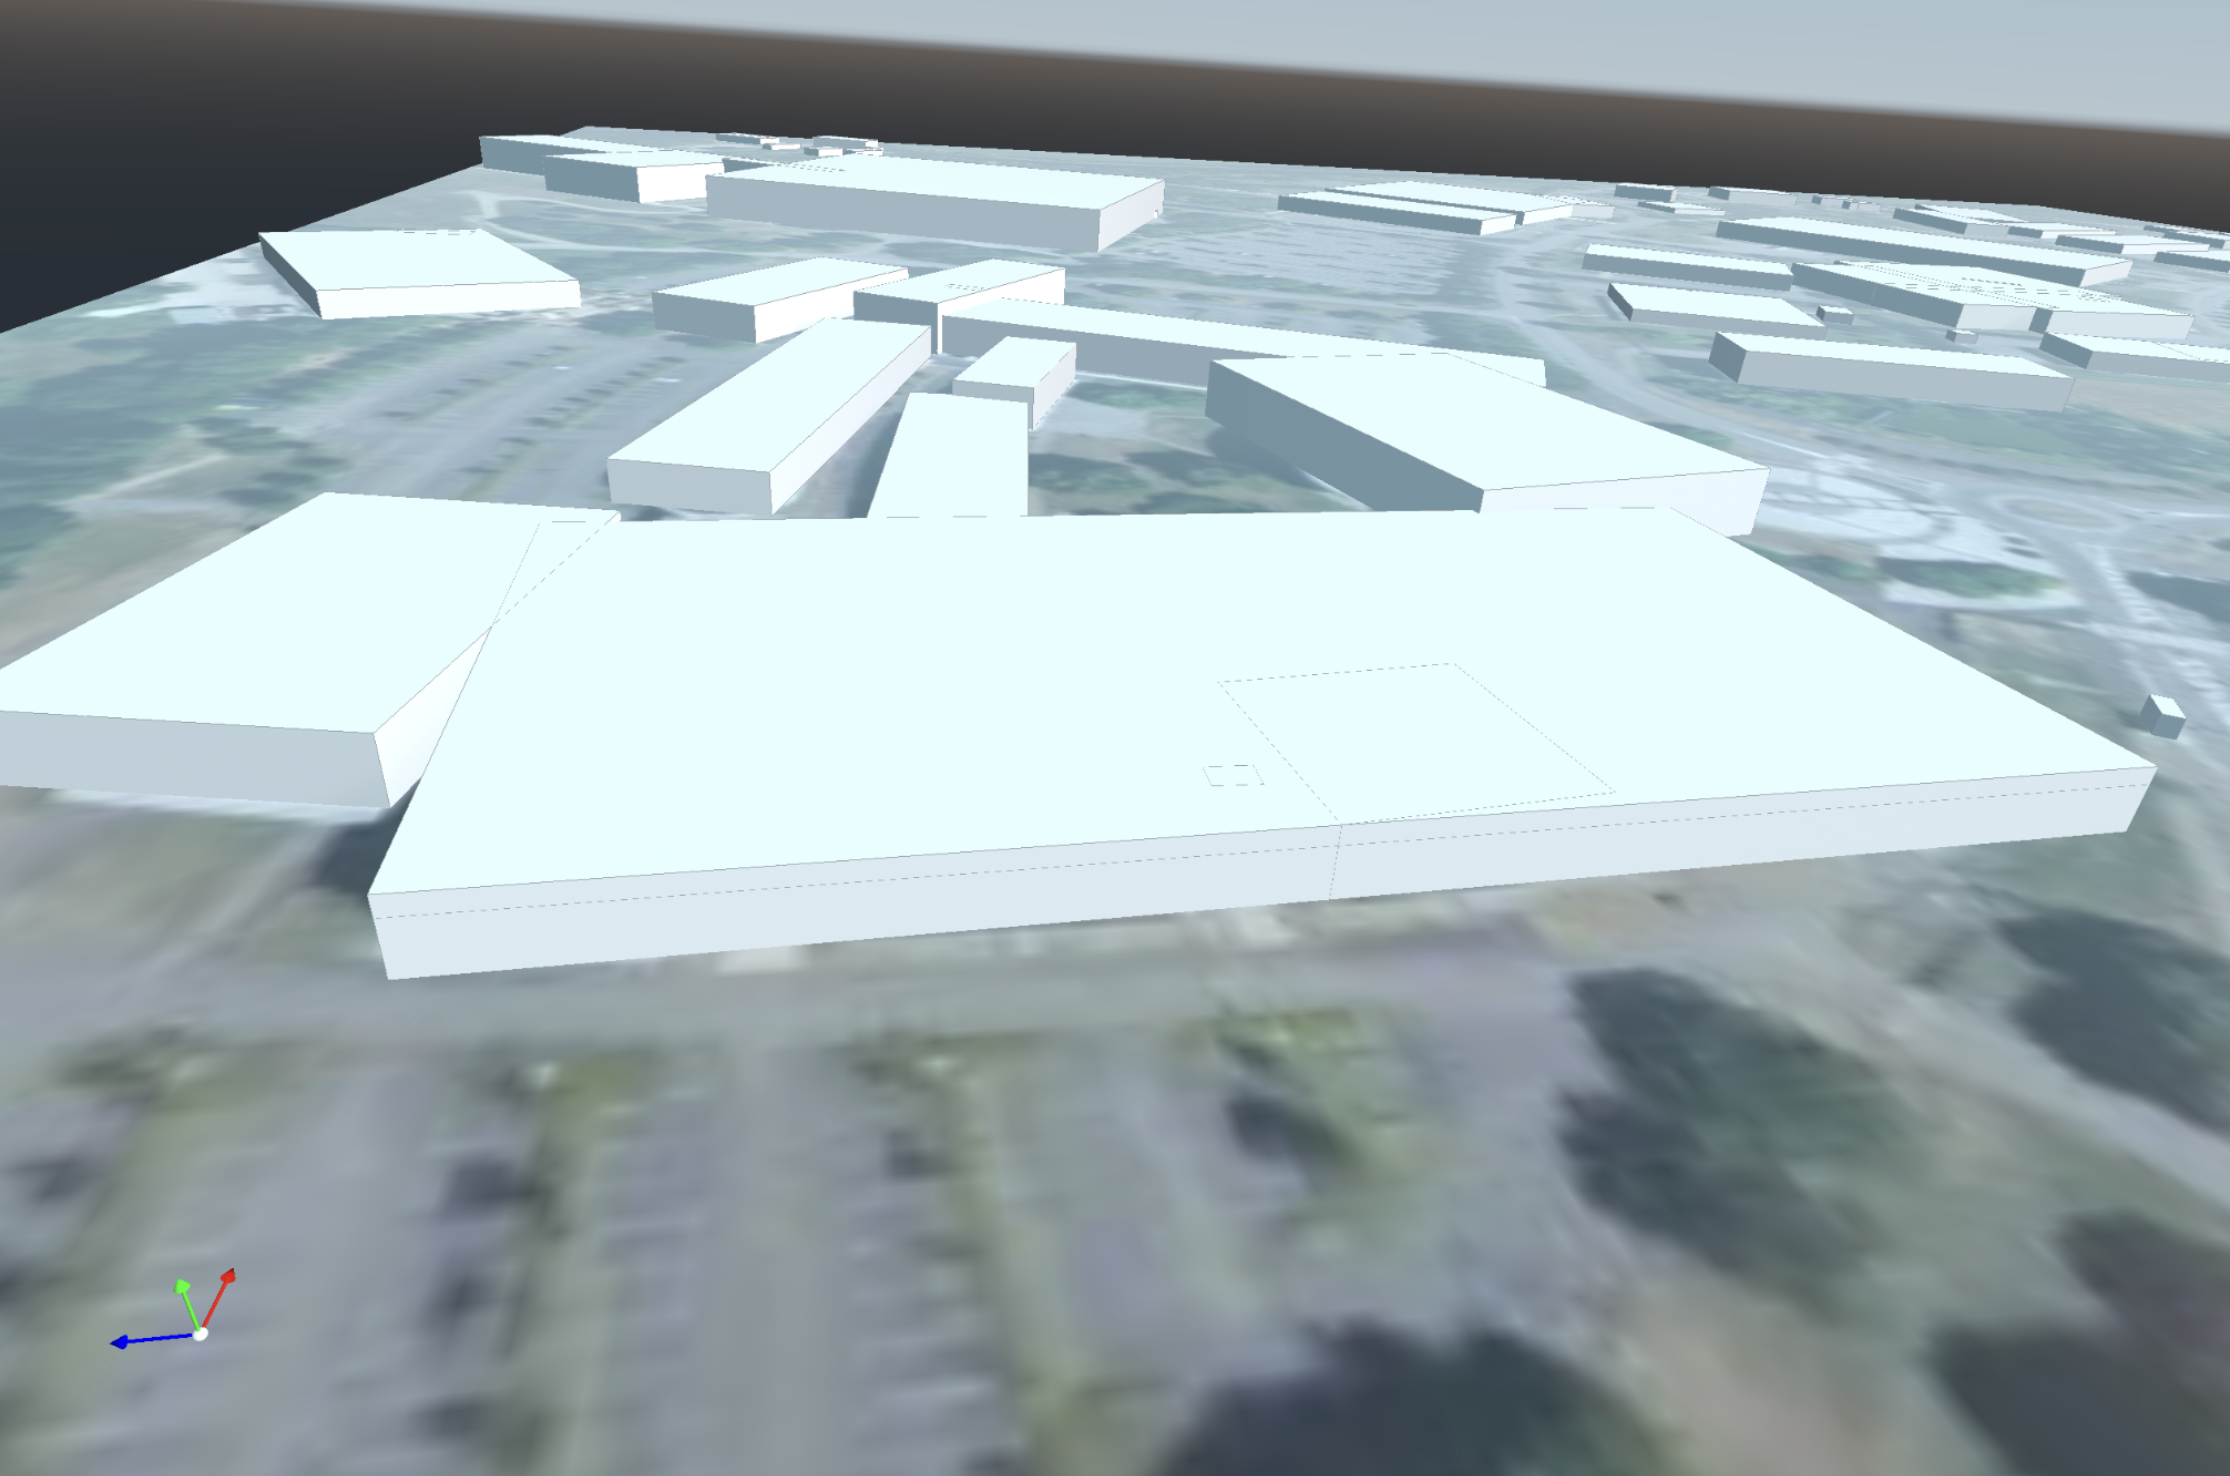
\includegraphics[width=\linewidth]{images/buildings-lod0.png}
  \caption{LOD-0: a building is represented by its bounding box}
  \label{fig:building-lod0}
\end{subfigure}%
\begin{subfigure}{.4\textwidth}
  \centering
  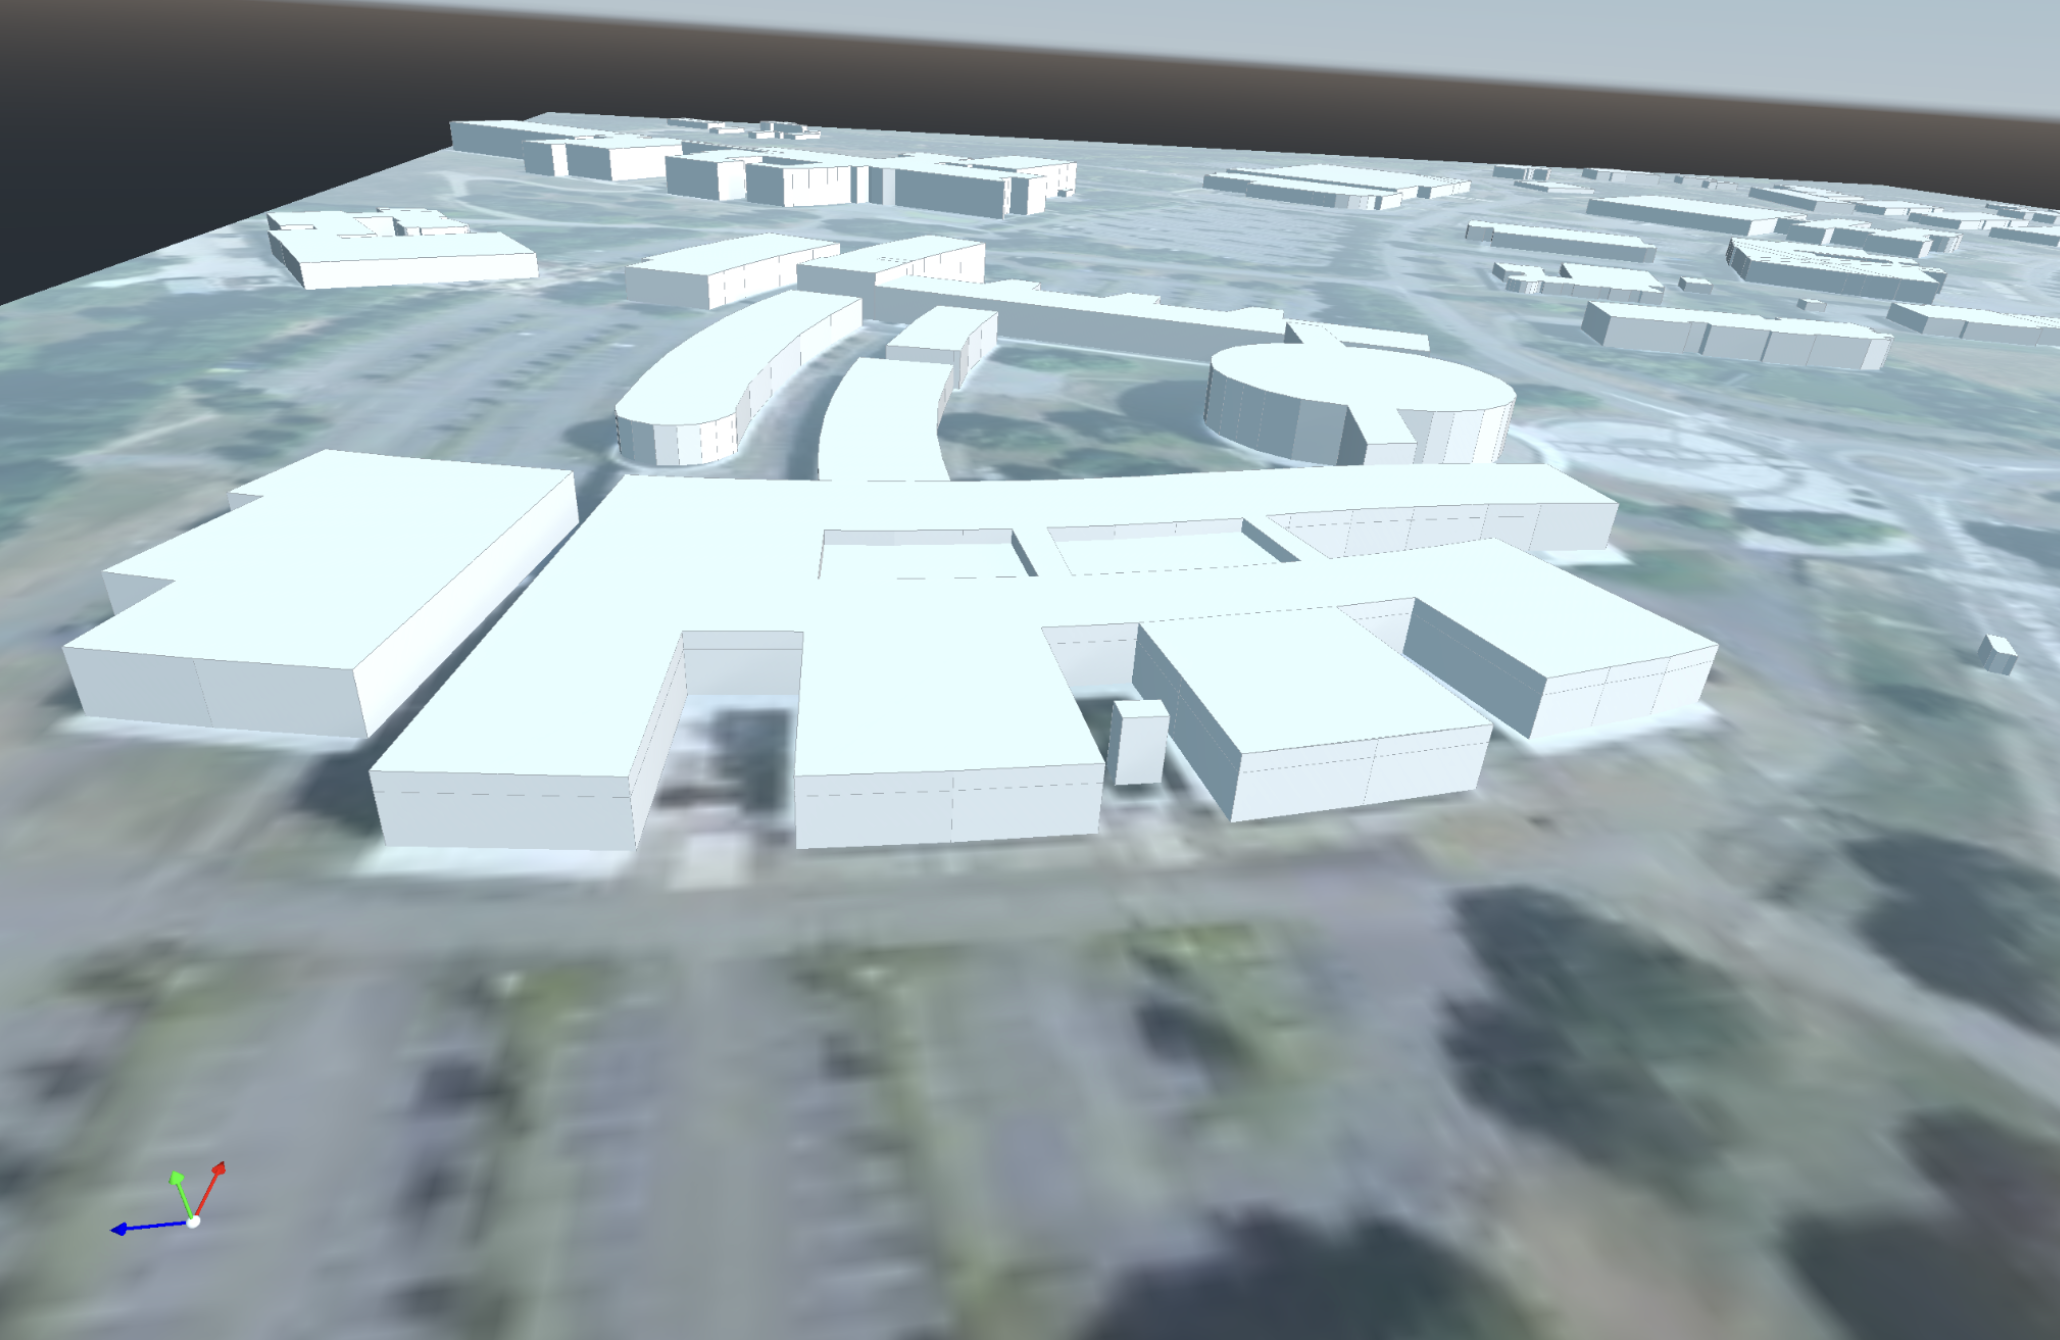
\includegraphics[width=\linewidth]{images/buildings-lod1.png}
  \caption{LOD-1: a building is represented by its ground footprint elevated to its height}
  \label{fig:building-lod1}
\end{subfigure}
\begin{subfigure}{.4\textwidth}
  \centering
  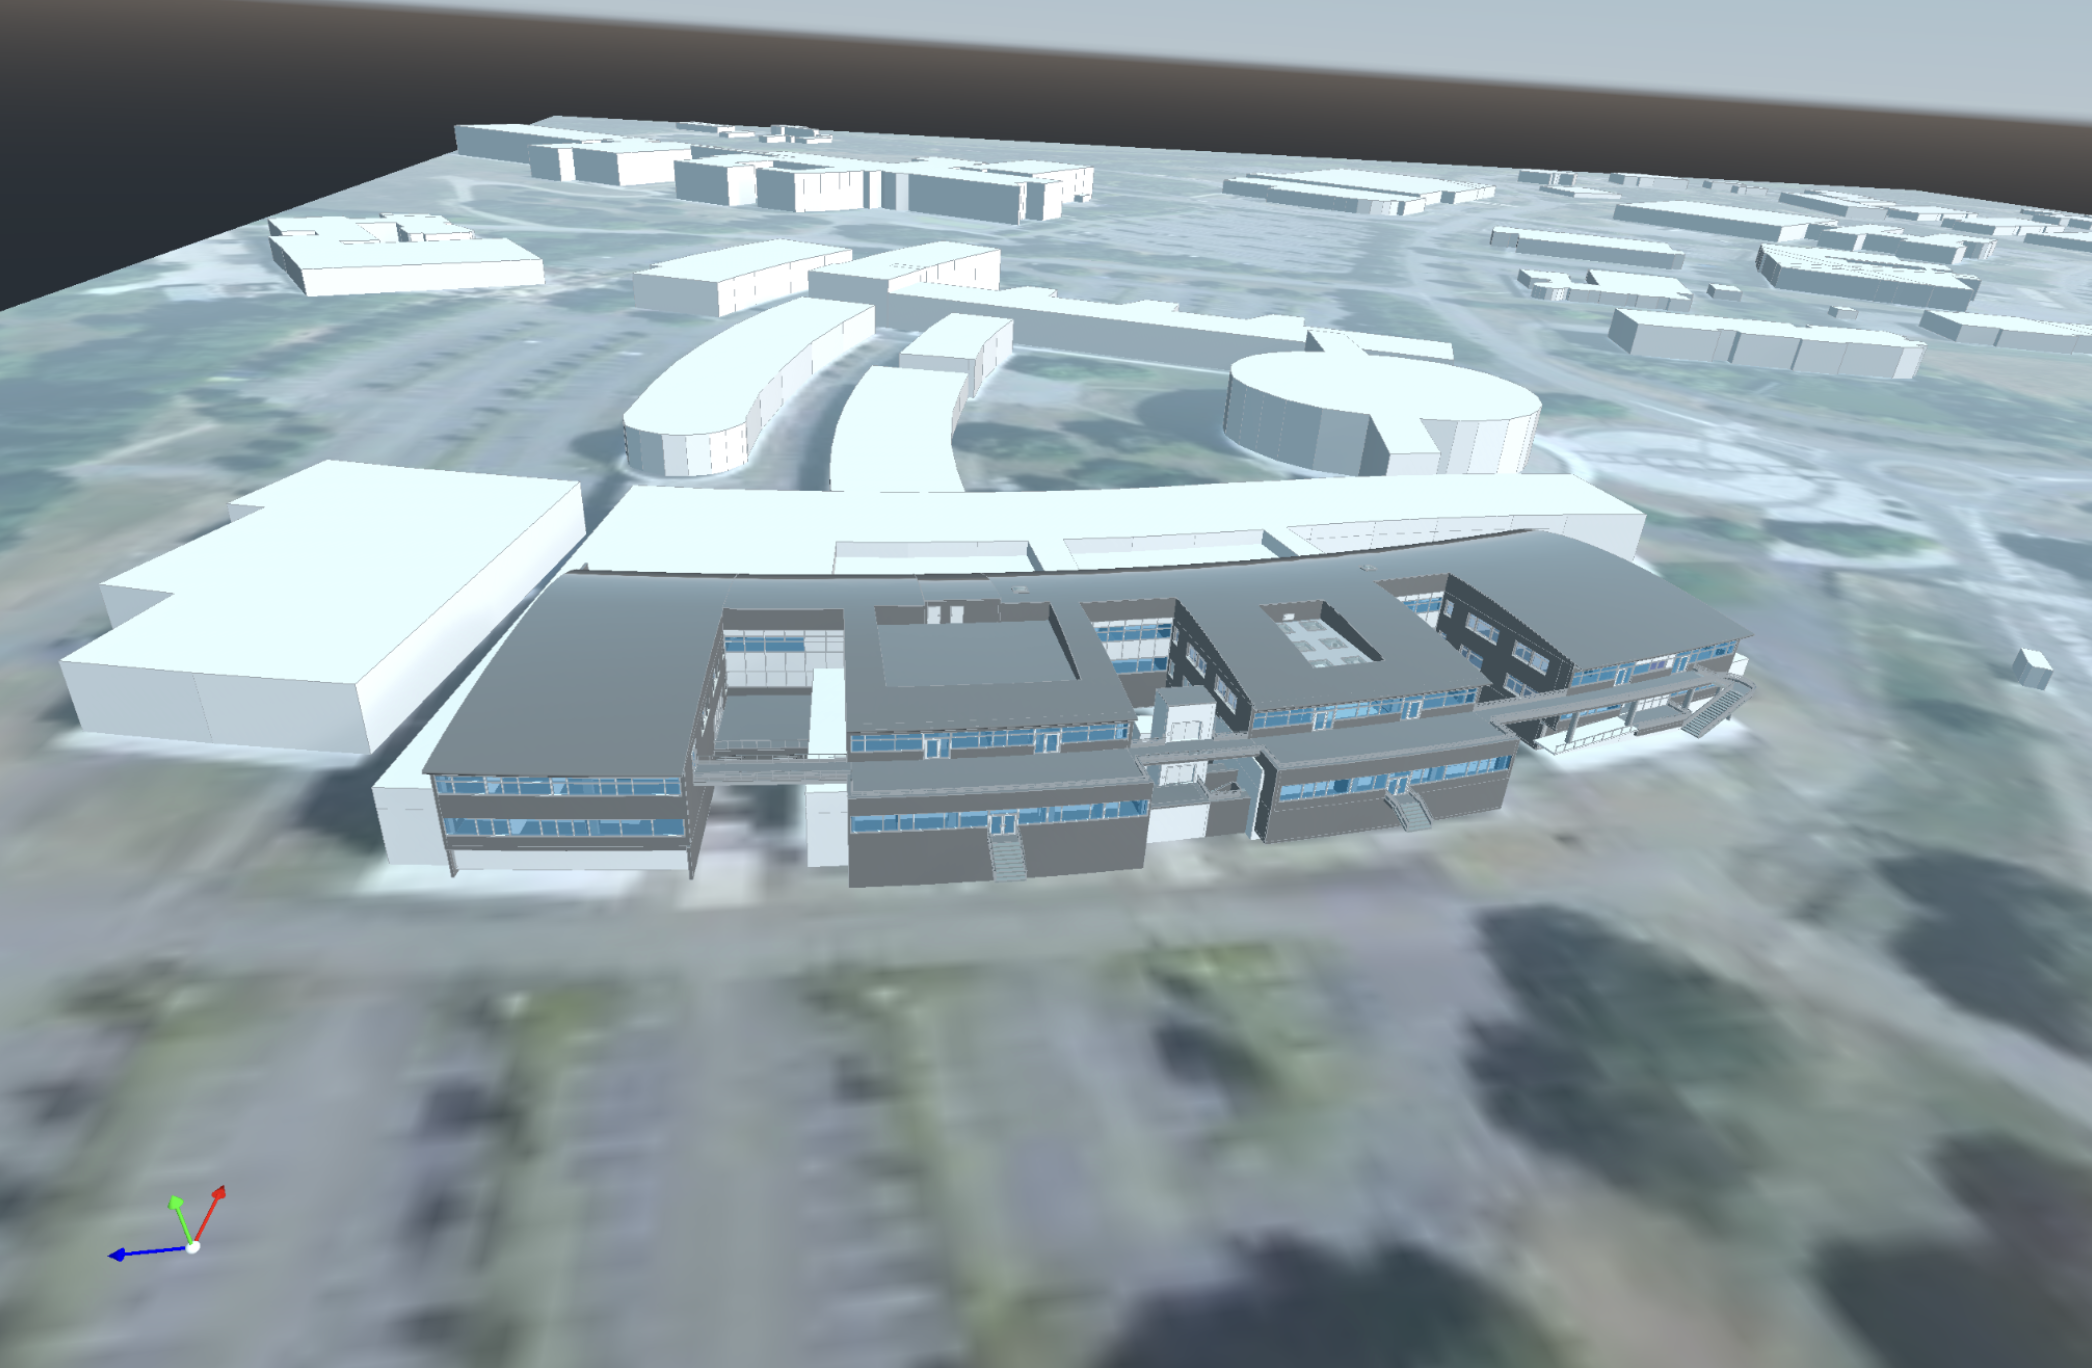
\includegraphics[width=\linewidth]{images/buildings-lod2.png}
  \caption{LOD-2: a building in full detail using BIM. Note that LOD-2 and LOD-1 are mixed.}
  \label{fig:building-lod2}
\end{subfigure}%
\begin{subfigure}{.4\textwidth}
  \centering
  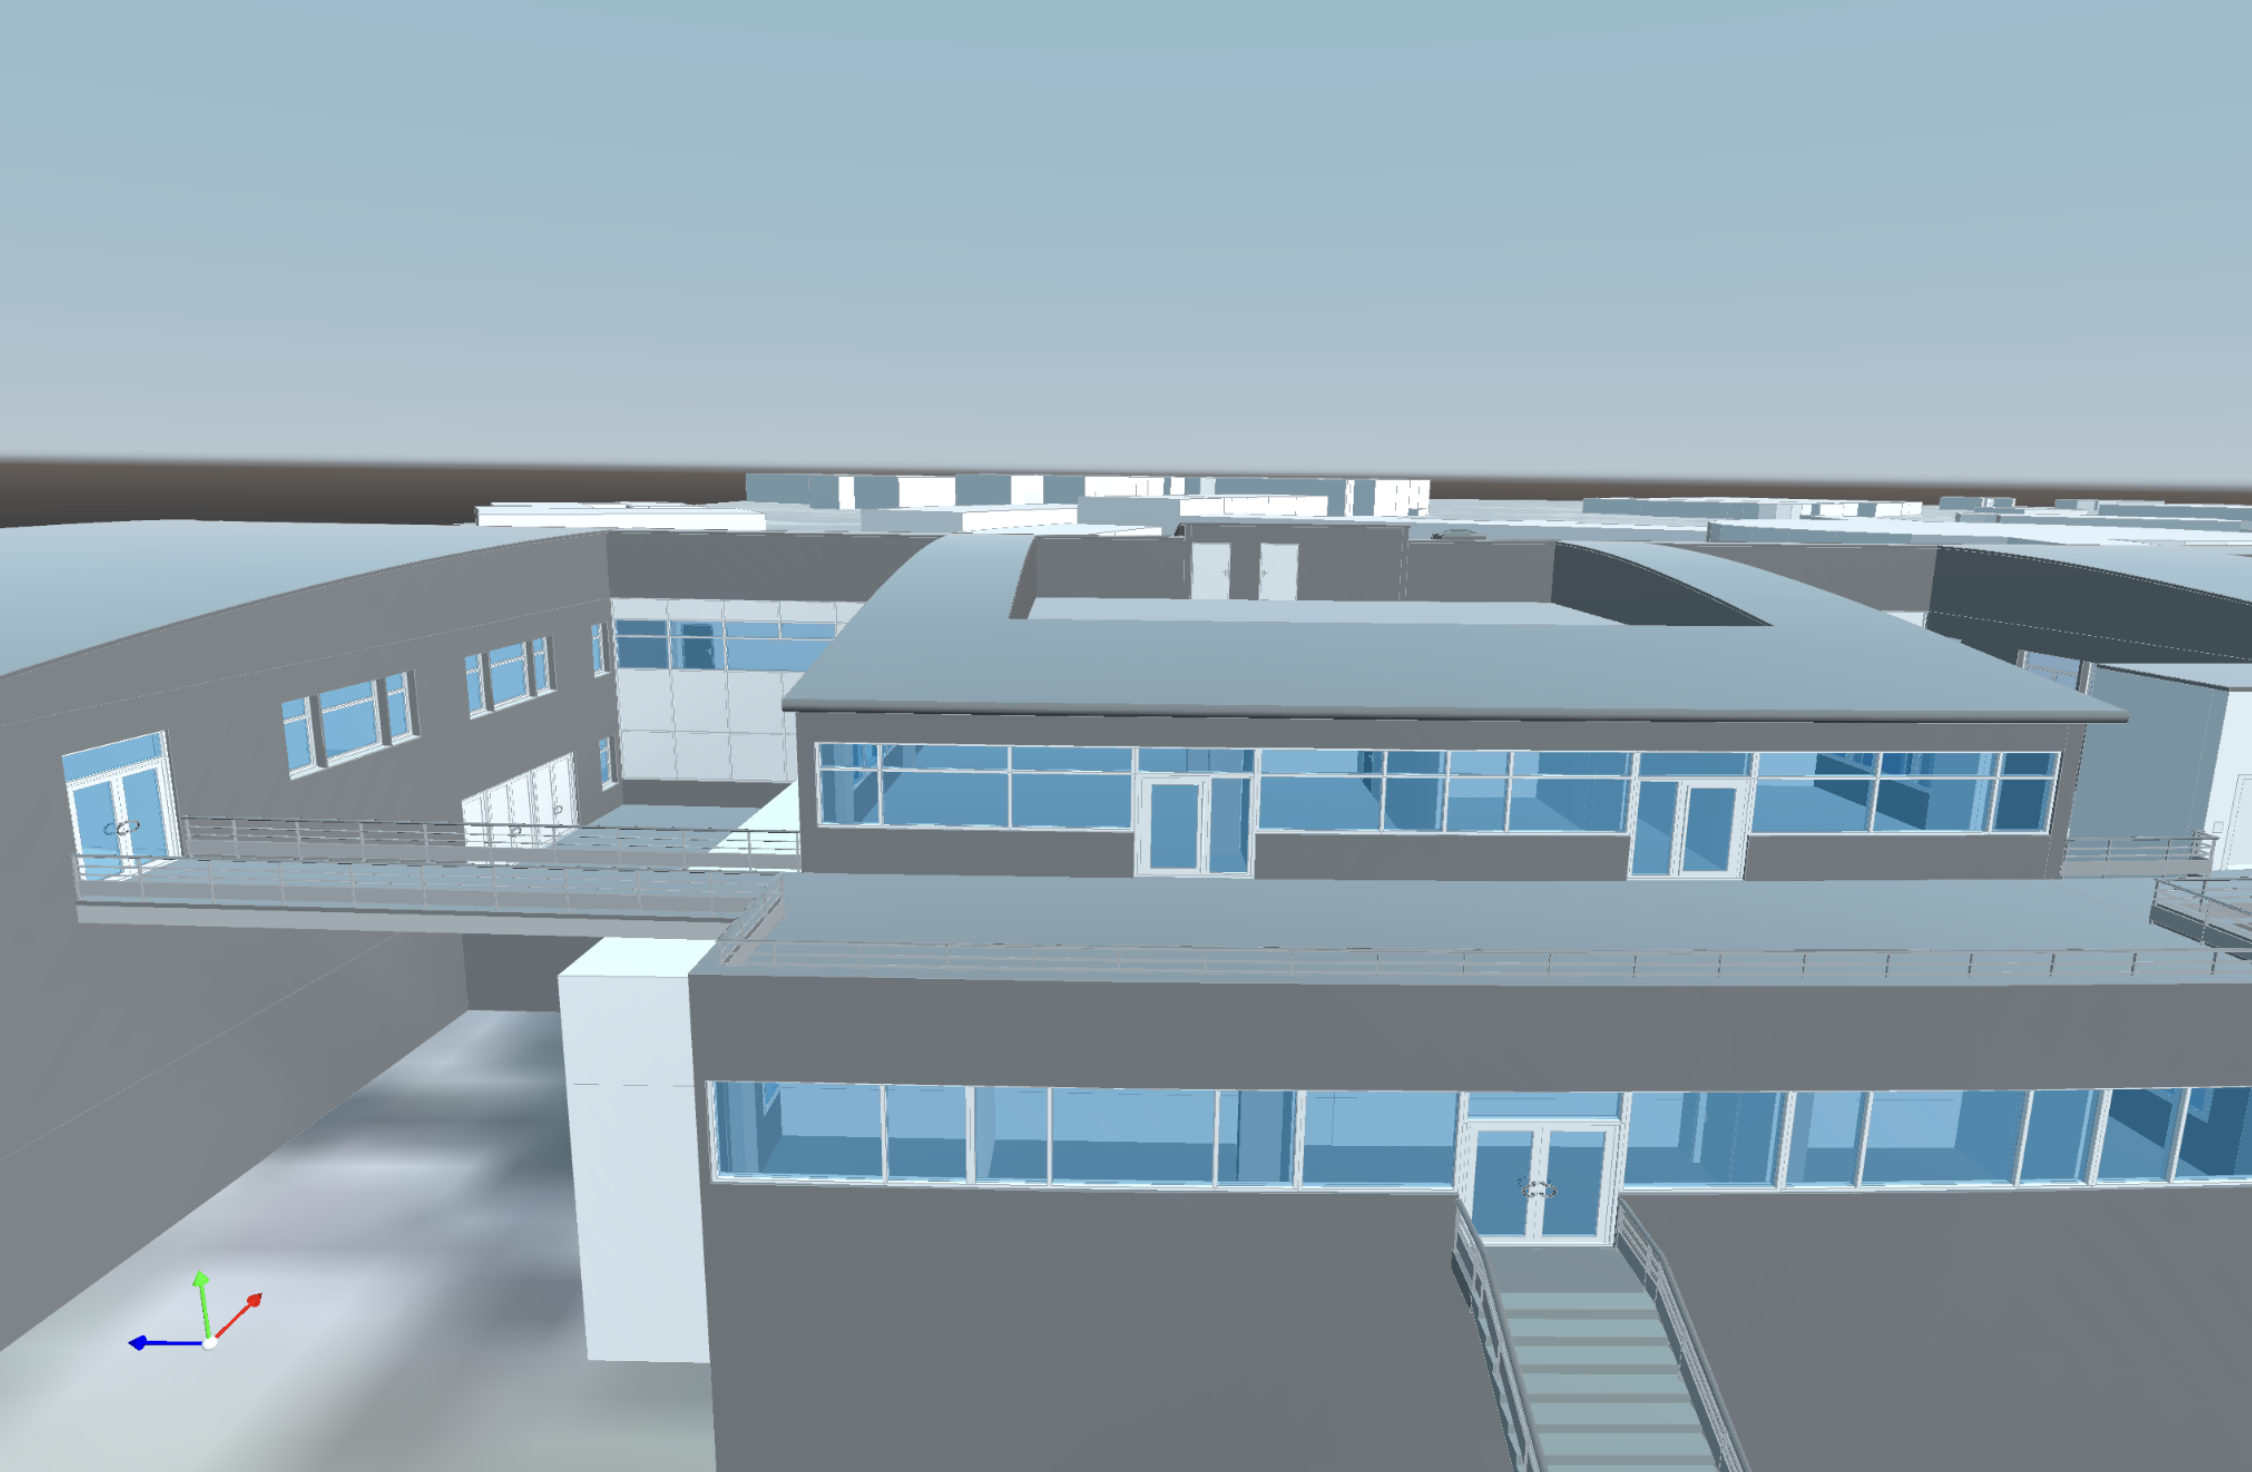
\includegraphics[width=\linewidth]{images/buildings-lod2-zoom.png}
  \caption{LOD-2: A zoom on the LOD-@ building.}
  \label{fig:building-lod2-zoom}
\end{subfigure}
\caption{Different representations of a building using our LOD definition}
\label{fig:buildings}
\end{figure}


Building meshes are generated from metadata fetched from web services like OpenStreetMap, which provides multi-polygons with holes, representing the complex urban fabric. For \textbf{LOD-0 and LOD-1}, buildings are modeled from 2D footprints extruded to form three-dimensional volumes. These volumes are then combined or subtracted to represent the district or the entire city, applying union operations on buildings that touch or intersect. In \textbf{LOD-2}, the focus shifts to creating conformal and watertight meshes that are suitable for detailed simulation tasks. These meshes are generated from Building Information Modeling (BIM) data in IFC format, enabling a detailed representation of each building component.

In the figure~\ref{fig:city-strasbourg}, we display an illustration of the center of the city of Strasbourg with LOD-0, see panel~\ref{fig:city-strasbourg-lod0}, and LOD-1, see panel~\ref{fig:city-strasbourg-lod1}, representations.

\subsubsection{Terrain Modeling}
The terrain modeling process utilizes elevation data extracted from raster images. The initial step involves creating a uniform mesh based on the size of the raster image. Following this, the elevation at each node is evaluated. Subsequently, isolines for elevation are computed, and mesh adaptation techniques are applied to reduce mesh density where feasible. Finally, each tile is glued together to ensure the continuity of the terrain mesh.

\subsubsection{Integration of Terrain and Building Meshes}
This process involves creating a conforming mesh that includes both the terrain and the buildings, ensuring that buildings on slopes are accurately modeled by adapting their height and embedding them into the terrain mesh. The figure~\ref{fig:city-grenoble-terrain} illustrates this aspect.

\subsubsection{Visual Representation}
Advanced rendering techniques are employed to visualize the multi-fidelity urban models, supporting both detailed analysis and general urban planning discussions. These visualizations are crucial for assessing the impact of urban changes and for stakeholder engagement.

This approach enhances the accuracy, utility, and scalability of urban models, making them vital for comprehensive urban analysis and planning in the HiDALGO2 project.

\begin{figure}[htbp]
\centering
\begin{subfigure}{.4\textwidth}
  \centering
  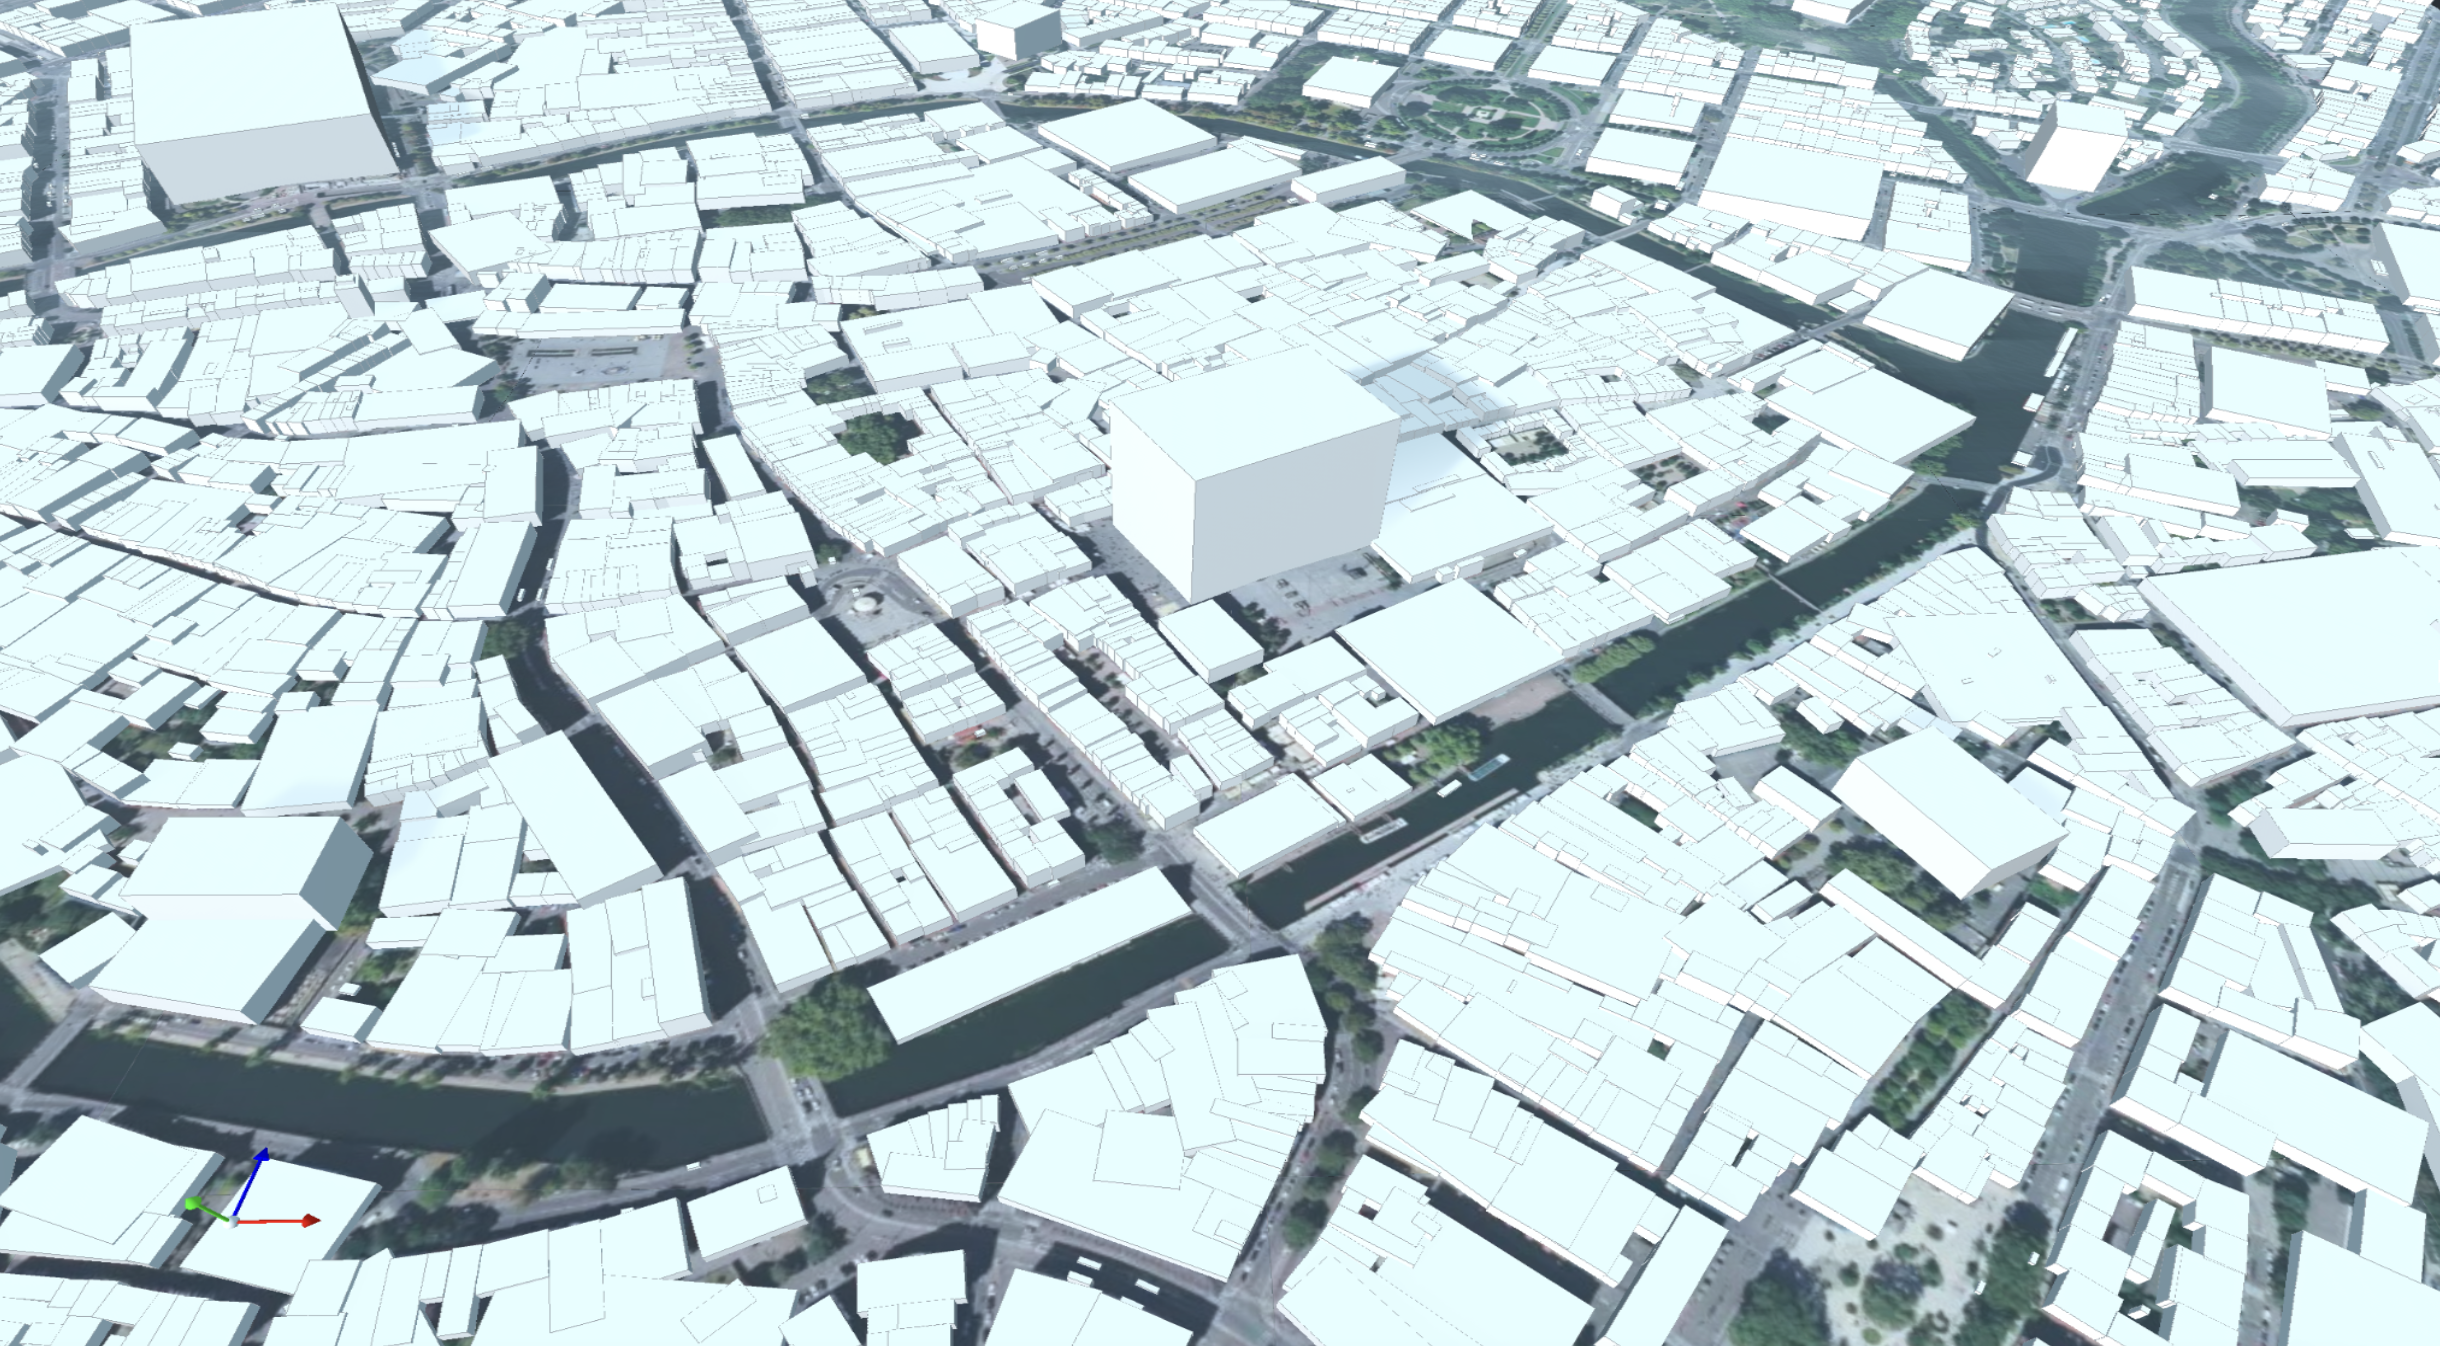
\includegraphics[width=\linewidth]{images/city-strasbourg-lod-0.png}
  \caption{LOD-0}
  \label{fig:city-strasbourg-lod0}
\end{subfigure}%
\begin{subfigure}{.4\textwidth}
  \centering
  \includegraphics[width=\linewidth]{images/city-strasbourg-lod-1.png}
  \caption{LOD-1}
  \label{fig:city-strasbourg-lod1}
\end{subfigure}
\begin{subfigure}{.4\textwidth}
  \centering
  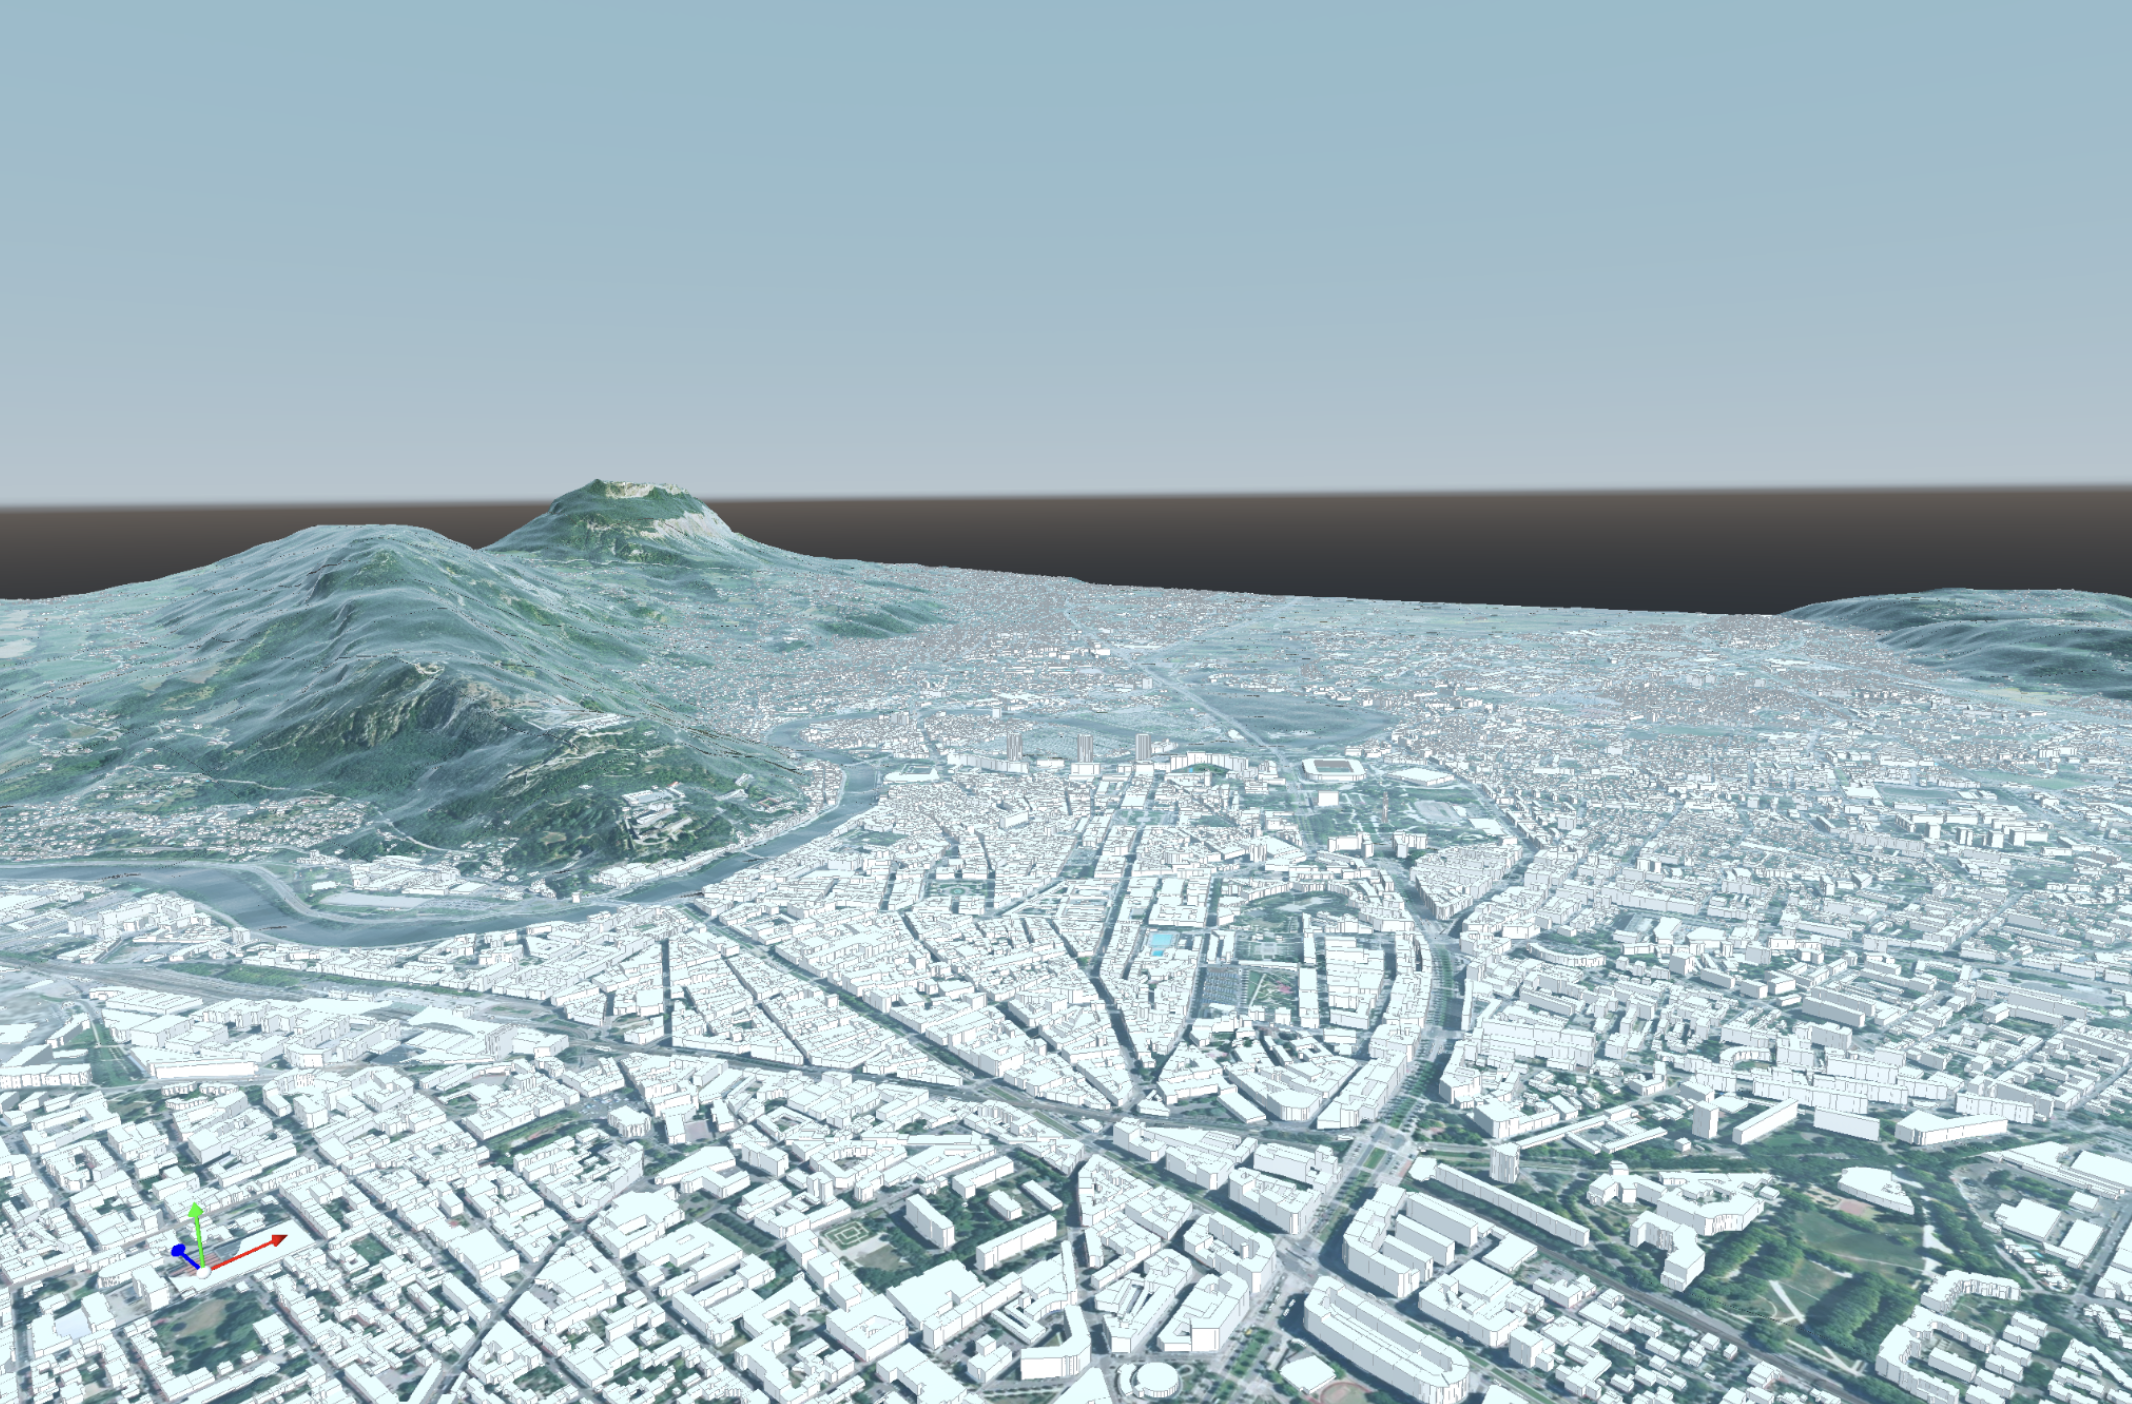
\includegraphics[width=\linewidth]{images/city-grenoble-terrain.png}
  \caption{LOD-1 terrain}
  \label{fig:city-grenoble-terrain}
\end{subfigure}
\caption{}
\label{fig:city-strasbourg}
\end{figure}

\subsubsection{Computational Tools for Building Meshes}

In the urban modeling process, particularly in the generation of building meshes, the Computational Geometry Algorithms Library (CGAL), plays a pivotal role. CGAL, \cite{the_cgal_project_cgal_2024} is renowned for its robust and efficient algorithms, which are crucial for handling complex geometric data and generating high-quality meshes from them.

\paragraph{Current Mesh Generation Strategy}
The current strategy for mesh generation employs multi-threading (MT) to handle various stages of the mesh construction process. Initially, the tiles to be used are determined based on the specified location, a task performed sequentially. Following this, GIS data, including buildings and elevation information, is downloaded in parallel. Next, polygons are repaired to ensure they are suitable for mesh generation, with this process executed in parallel using MT. The terrain mesh is then generated in parallel, employing CGAL's algorithms to ensure precision and efficiency. Union operations at tile junctions are performed to ensure continuity, a step that is currently sequential. Finally, building meshes are generated using a parallel MT approach, leveraging CGAL for its advanced mesh generation capabilities.

\paragraph{Advancing Towards Full Parallelism}
The next steps in enhancing the mesh generation process involve moving towards a fully parallel approach using both Multi-threading (MT) and Message Passing Interface (MPI). The goal is to scale the process up to handle entire cities or larger urban areas. This scale-up involves utilizing MPI to manage distributed computing resources effectively. To achieve this, partitions of tiles with overlapping areas are created to ensure complete and accurate building descriptions without the need for extensive MPI communication. Furthermore, each process uses an MT strategy to generate meshes independently, with overlapping zones allowing for the creation of complete building structures.

\subsubsection{Partitioning Strategies Depending on Simulation Use Cases}
Different partitioning strategies are employed depending on the specific requirements of the simulation use cases. For simple scenarios where buildings do not interact with their environment, a basic listing and weighting strategy is sufficient, known as Test Case 0. In Test Case 1, where buildings interact with environmental elements, a more complex partitioning strategy is necessary that considers both the buildings and their immediate non-building surroundings. For full interaction models, as in Test Case 2, the partitioning strategy starts with the buildings and extends to the entire urban mesh, ensuring that all elements are considered to minimize communication overhead. Looking towards scenarios with extreme partitioning needs, Test Case 3 employs a multigrid approach, defining coarse and fine meshes to efficiently manage computational resources. This multi-fidelity approach not only enhances the accuracy and applicability of urban models in simulations but also ensures scalability across different computational platforms, making it a cornerstone of urban analysis in the HiDALGO2 project.

The figure~\ref{fig:partitioning} illustrates the different strategies discussed previously and present a reconstruction of New York with 10km square reconstruction with hundreds of thousands of buildings which requires the large scale approach discussed but not yet implemented nor tested.
\begin{figure}[htbp]
\centering
\begin{subfigure}{.4\textwidth}
  \centering
  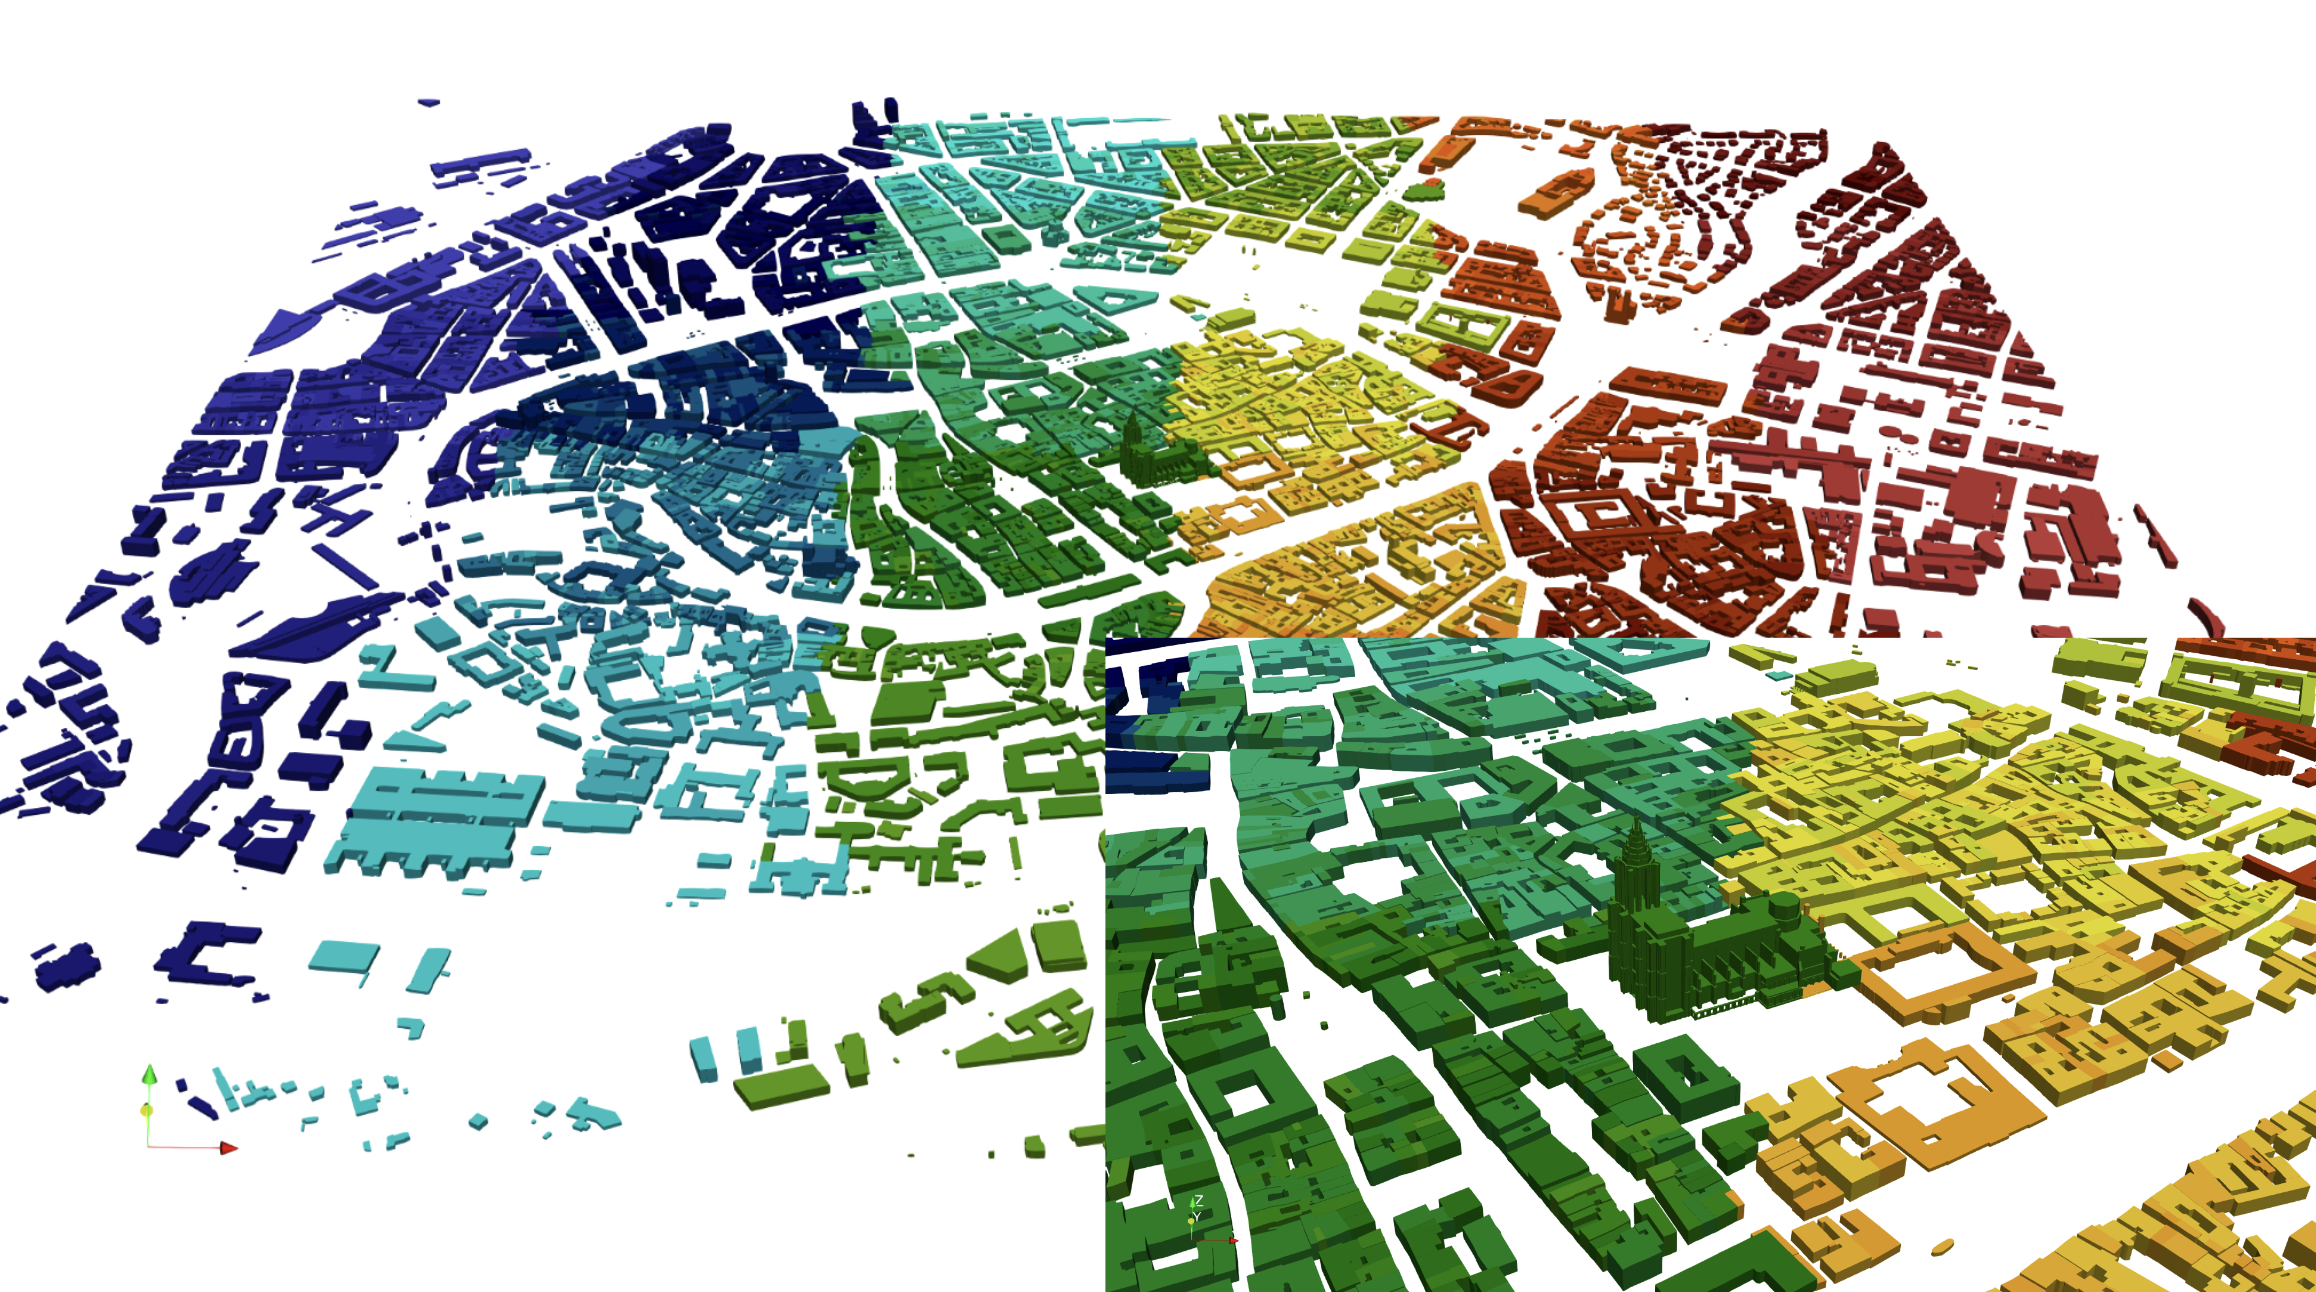
\includegraphics[width=\linewidth]{images/city-strasbourg-lod0-parts.png}
  \caption{LOD-0}
  \label{fig:city-strasbourg-lod0-parts}
\end{subfigure}%
\begin{subfigure}{.4\textwidth}
  \centering
  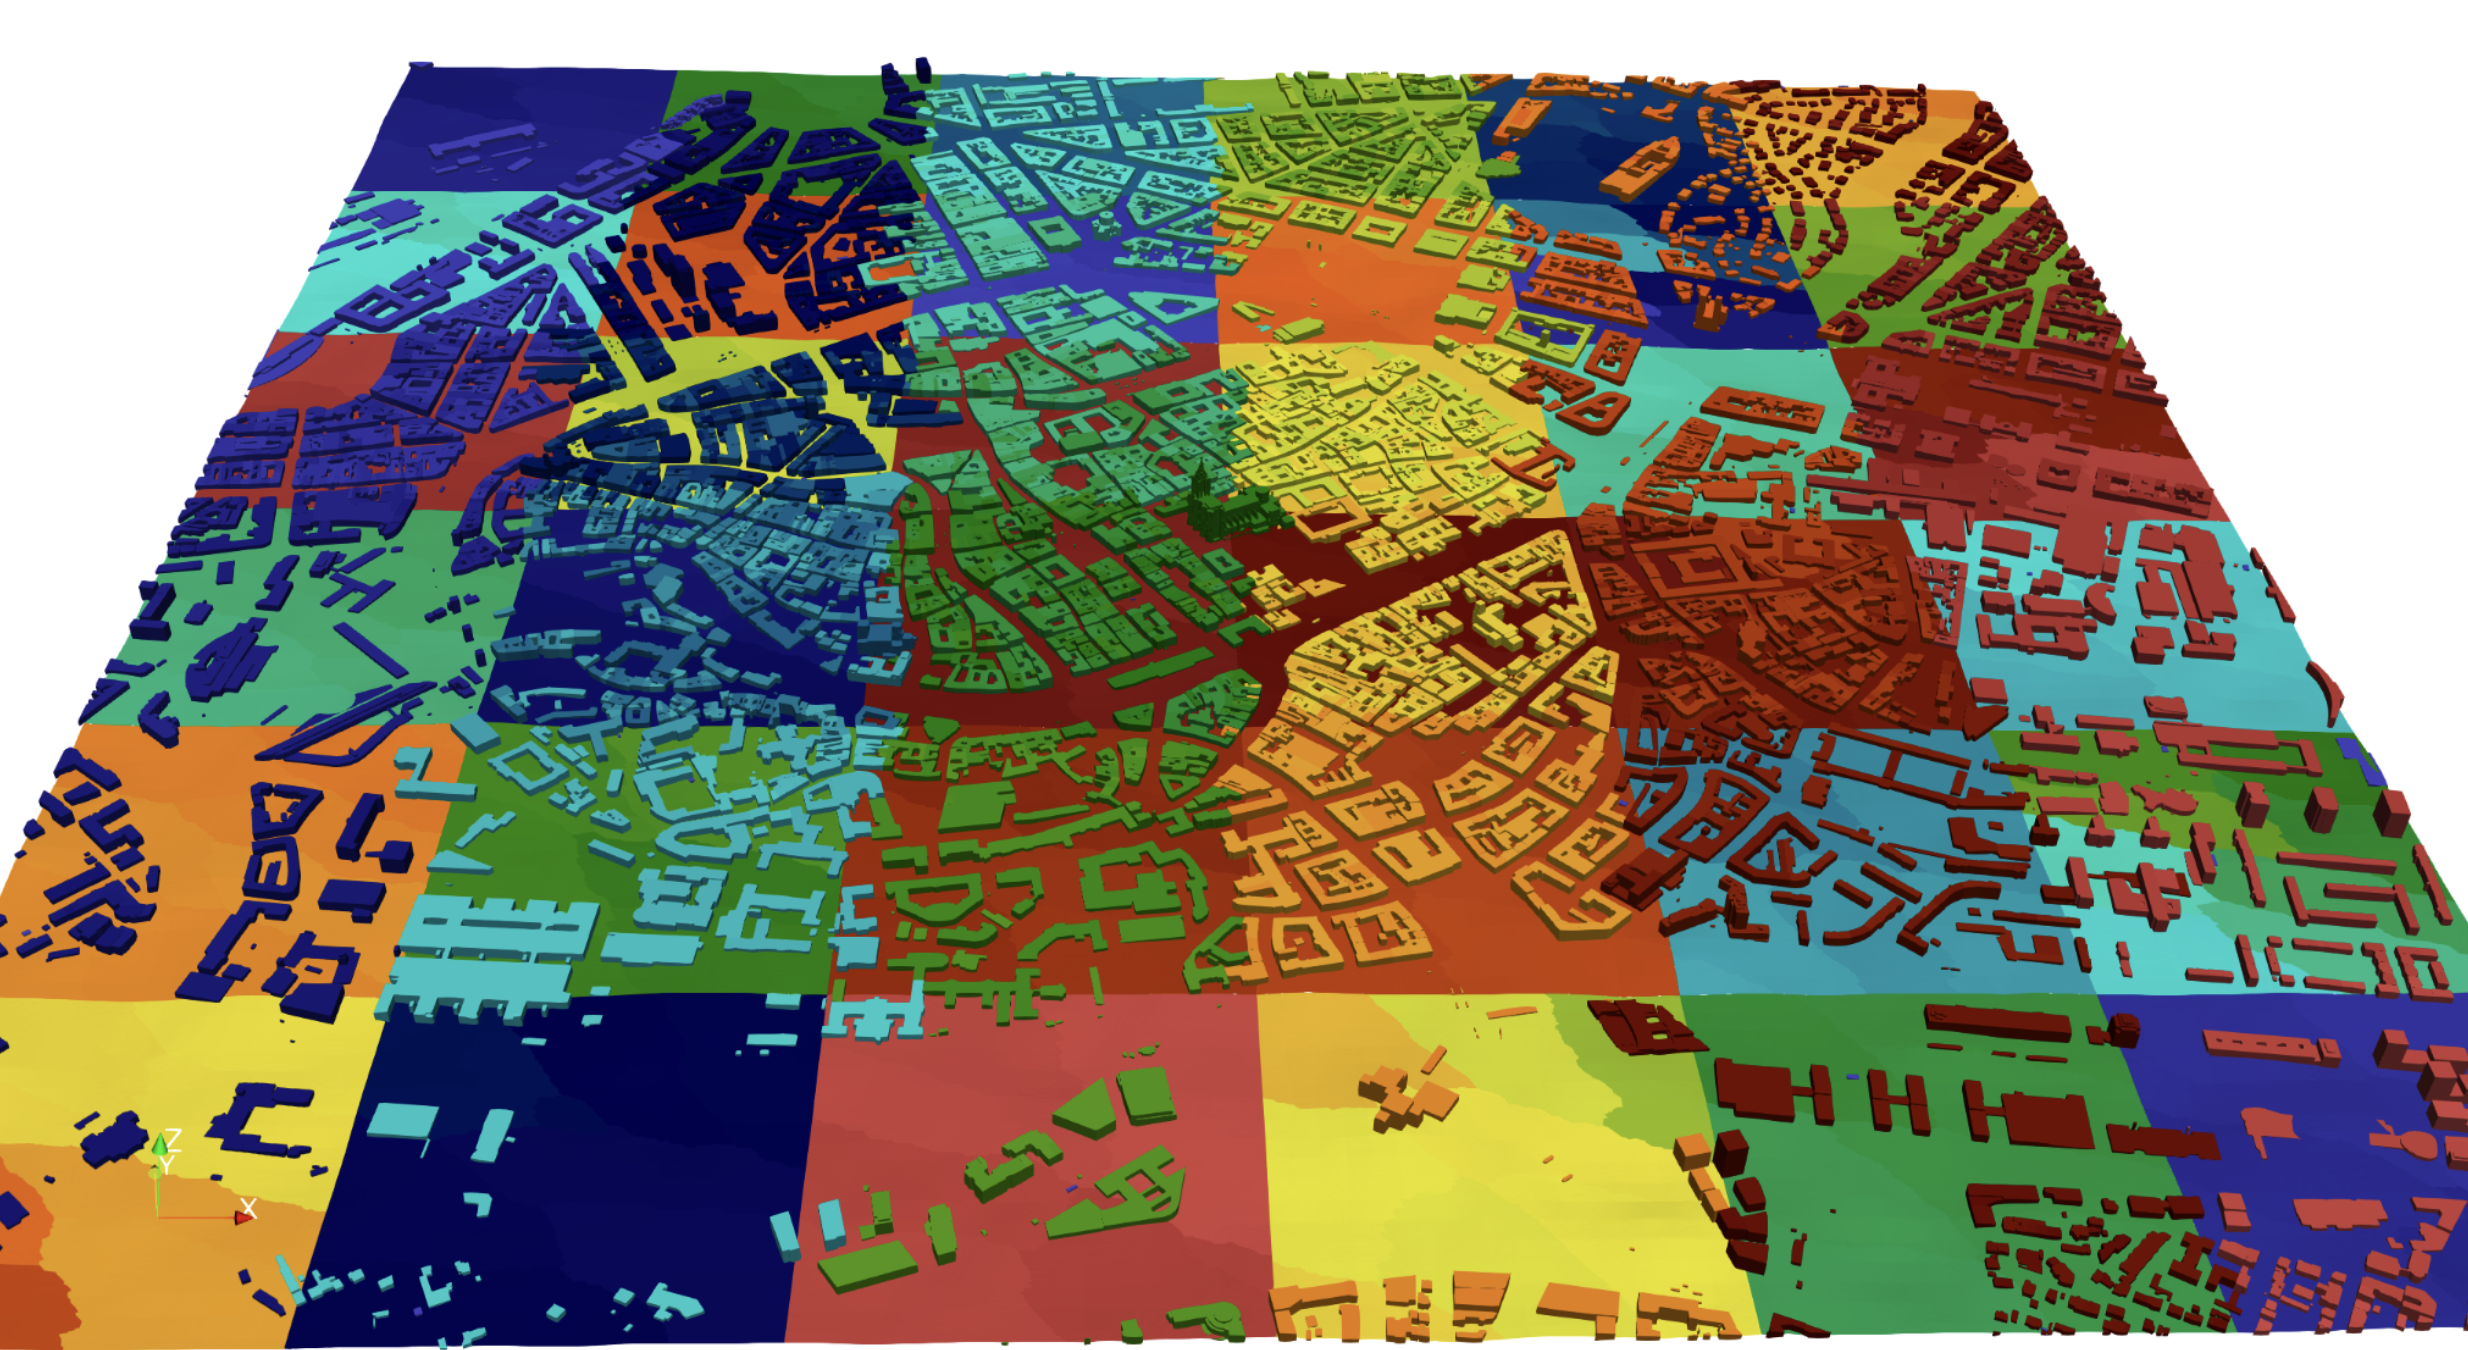
\includegraphics[width=\linewidth]{images/city-strasbourg-lod1-parts.png}
  \caption{LOD-1}
  \label{fig:city-strasbourg-lod1-parts}
\end{subfigure}
\begin{subfigure}{.4\textwidth}
  \centering
  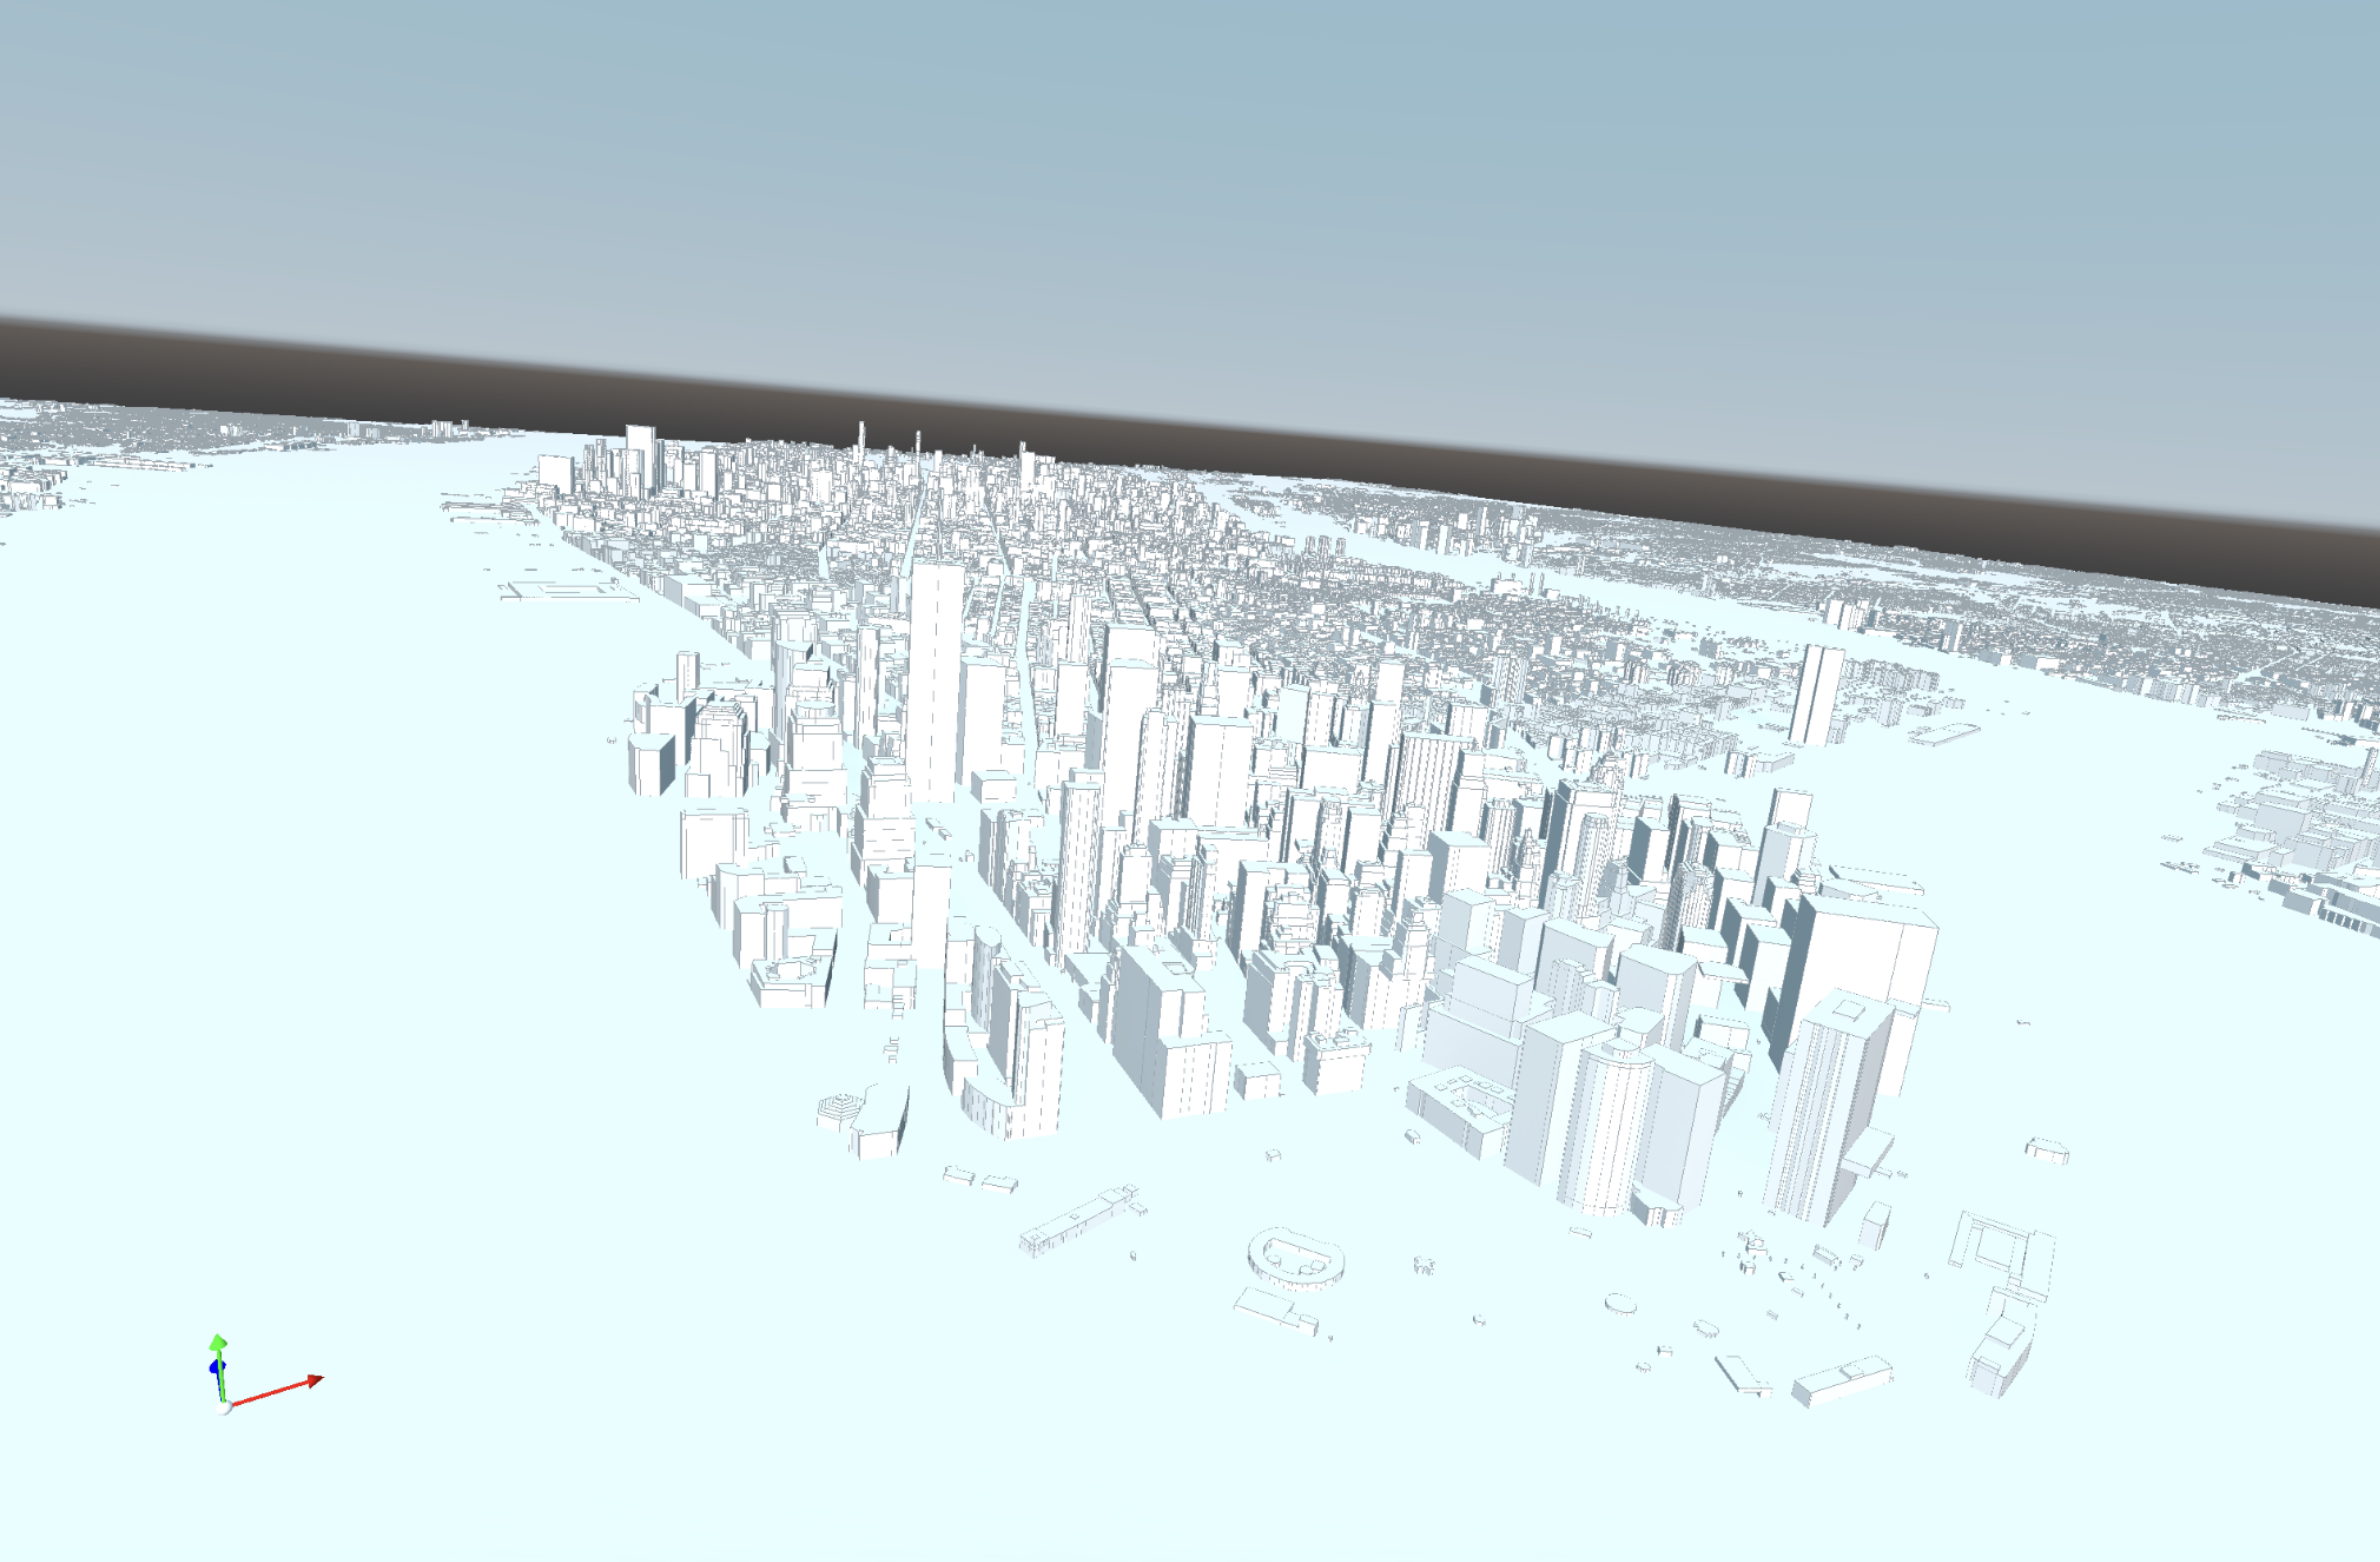
\includegraphics[width=\linewidth]{images/city-newyork-largescale.png}
  \caption{LOD-1 Large scale}
  \label{fig:city-ny-largescale}
\end{subfigure}
\caption{}
\label{fig:partitioning}
\end{figure}

\subsubsection{Conclusion on mesh construction}
Our strategy not only aims to improve the efficiency and scalability of the mesh generation process but also enhances the fidelity and accuracy of the urban models used in simulations.

\subsection{Modeling and simulations}

We now turn to describing the physical modeling of city energy simulation.
To do this, we built on two main tools: Feel++ and Modelica. 

\subsubsection{Feel++ Toolchain}

Feel++ is a comprehensive framework designed to tackle problems based on Ordinary Differential Equations (ODEs) and Partial Differential Equations (PDEs). Using modern C++ (C++17 and C++20) standards coupled with a Python layer through Pybind11, Feel++ enables seamless parallelism and is equipped with default communicators that simplify handling complex computational tasks. The framework's versatility is evident in its deployment across various platforms, including research and educational environments and cloud services tailored for high-performance computing needs.

Key features of the Feel++ framework encompass an extensive range of numerical methods designed to address Partial Differential Equations (PDEs). These methods include continuous Galerkin (cG), discontinuous Galerkin (dG), hybrid discontinuous Galerkin (hdG), and reduced basis methods (rb/mor). A Domain Specific Language (DSL) for Galerkin methods significantly enhances the ease of implementing and experimenting with new numerical methods. The de Rham complex provides a comprehensive toolkit for constructing finite element spaces of arbitrary order, facilitating precise mathematical modeling. The framework's automatic differentiation and symbolic integration capabilities effectively bridge the gap between mathematical expressions and their computational implementation. Feel++ supports diverse applications from fluid dynamics and structural mechanics to heat transfer and electrostatics, demonstrating its flexibility and broad applicability. Furthermore, its integration with Specx for task-based parallel execution optimizes performance and scalability on modern computational architectures.

\paragraph{Simulation Tools and Applications}
Feel++ comes equipped with a variety of toolboxes tailored for specific application domains, offering pre-built scenarios for fluid dynamics, solid mechanics, and electromagnetism, among others. These toolboxes are designed to provide robust and efficient solutions, leveraging the capabilities of Feel++ to address complex multi-physics problems in real-world scenarios.

Documentation and further details can be accessed through Feel++ Toolboxes Documentation\footnote{\url{https://docs.feelpp.org/toolboxes/latest/}}.
This powerful toolchain is essential for the Urban Building pilot of the HiDALGO

\subsubsection{Computing Shading Masks and View Factors with Feel++}

In urban building energy simulations, the computation of shading masks and view factors is crucial for accurately modeling the impact of solar radiation on building surfaces. Shading masks quantify the percentage of blocked solar radiation for each building surface (including walls and roofs) depending on the direction of the sun. This is influenced by nearby structures such as other buildings, vegetation, and urban furniture. The view factors describe the fraction of radiation that leaves one surface and strikes another, which are essential for calculating radiative heat exchanges between building surfaces.

\paragraph{Numerical Methods and Challenges}
Both shading masks and view factors are computed using Monte Carlo and ray tracing techniques, which allow for handling complex geometries with various obstructions. Despite being purely geometric quantities, these calculations face significant challenges such as:
\begin{itemize}
    \item Efficient computation of integrals for view factors, especially when considering specular surfaces that require multiple ray bounces.
    \item Managing large-scale mesh computations and data storage, particularly when detailed urban environments are modeled.
\end{itemize}

\paragraph{Implementation in Feel++}
Feel++ facilitates these computations through its robust numerical methods optimized for high performance and parallel execution. For each face of a building, Feel++ computes solar masks using a Monte Carlo approach for various sun positions, ensuring efficient and scalable processing across multiple CPU cores. This enables the integration of dynamic solar shading effects into the simulation of building energy performance, providing a more accurate representation of real-world conditions.

\begin{figure}[htbp]
\centering
\begin{subfigure}{.4\textwidth}
  \centering
  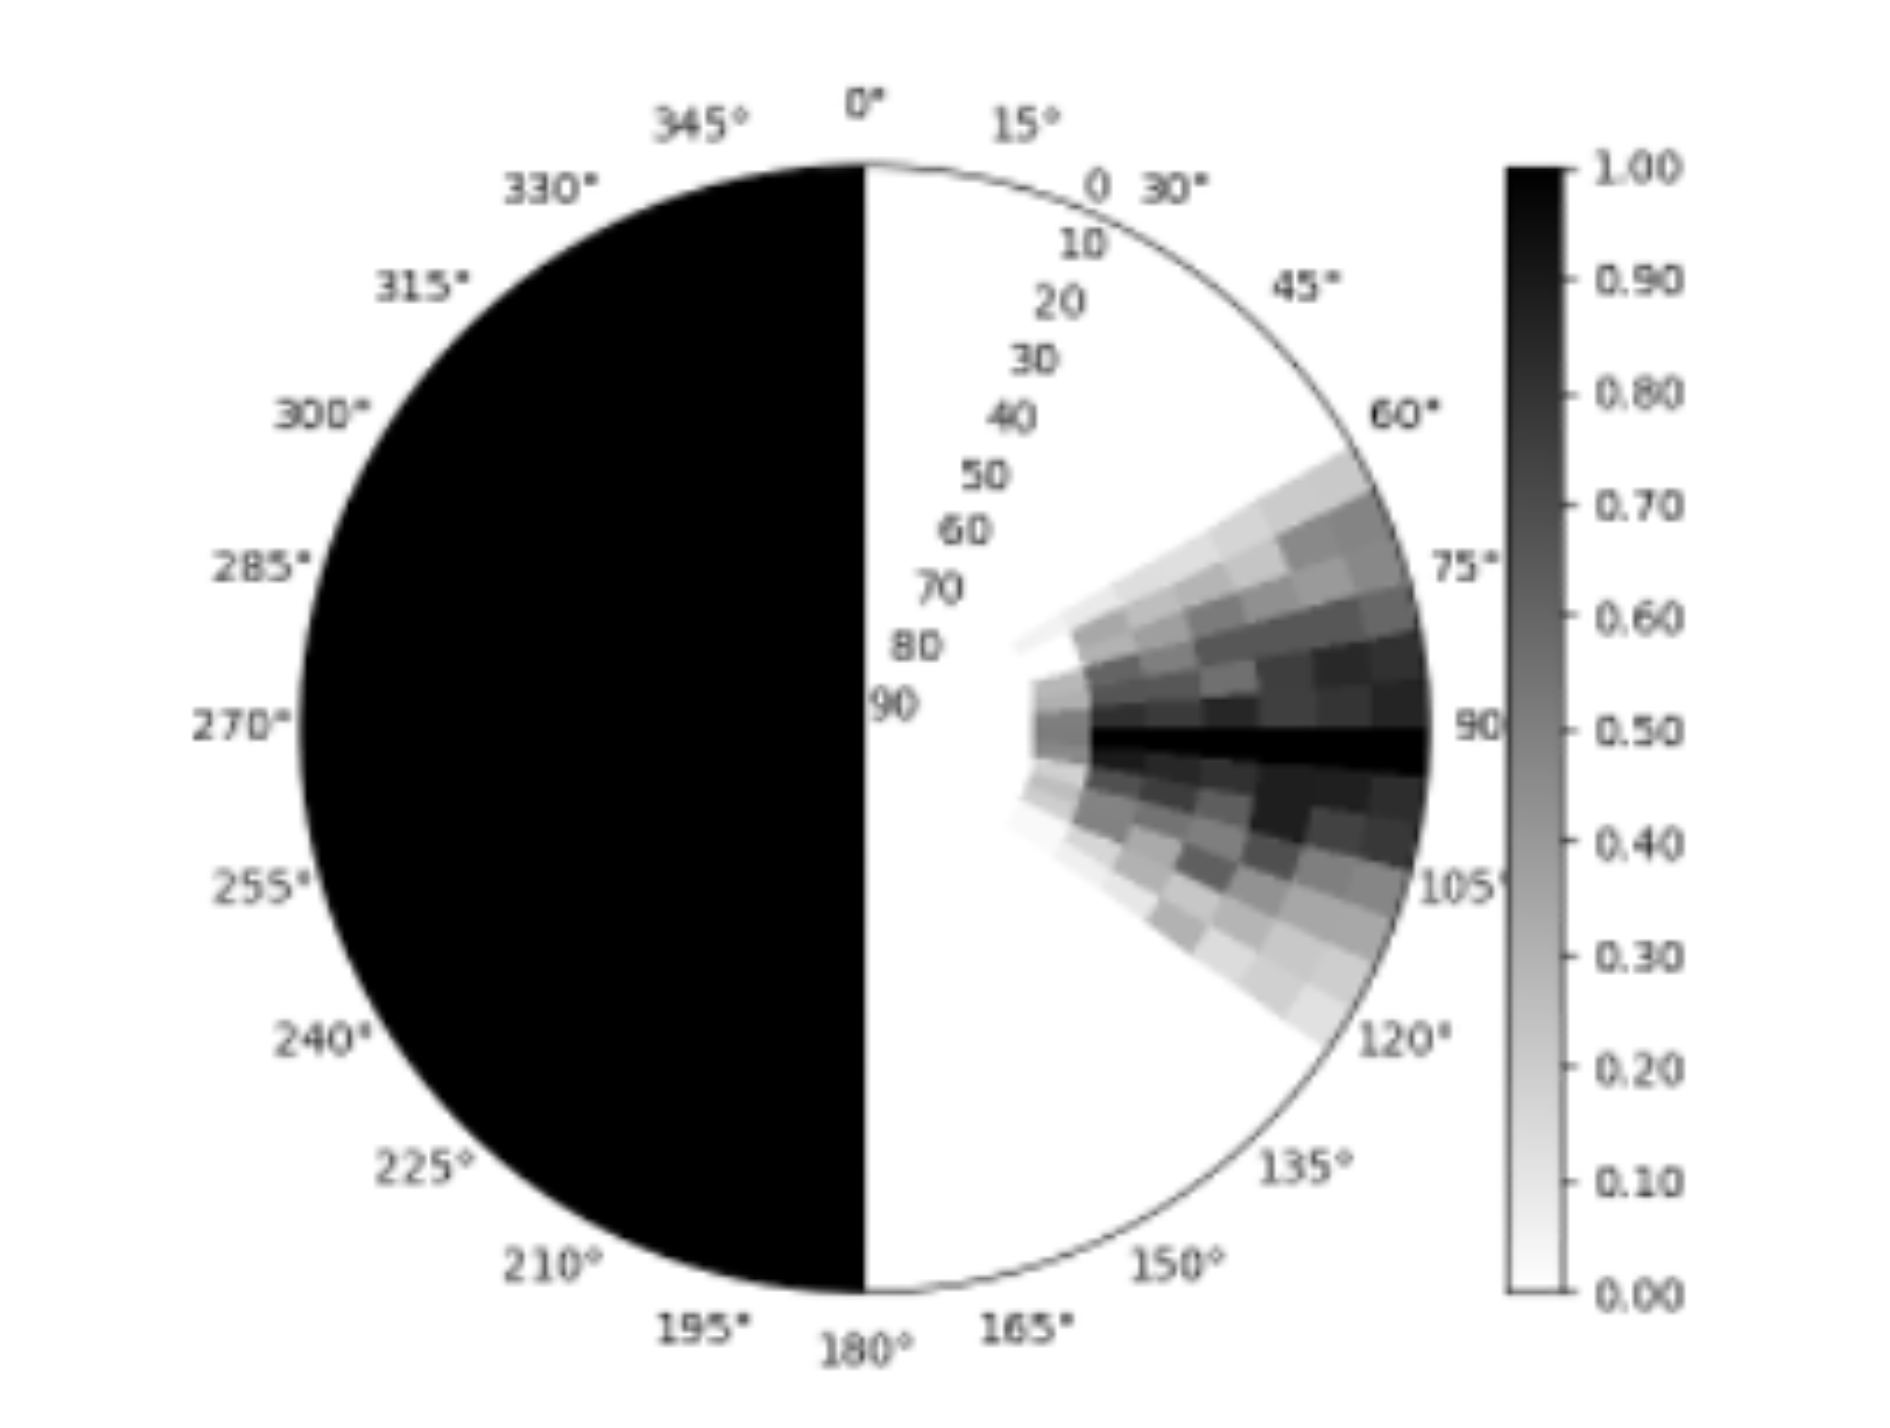
\includegraphics[width=\linewidth]{images/solar-masks-east-facing.png}
  \caption{LOD-0}
  \label{fig:sm-building-east}
\end{subfigure}%
\begin{subfigure}{.4\textwidth}
  \centering
  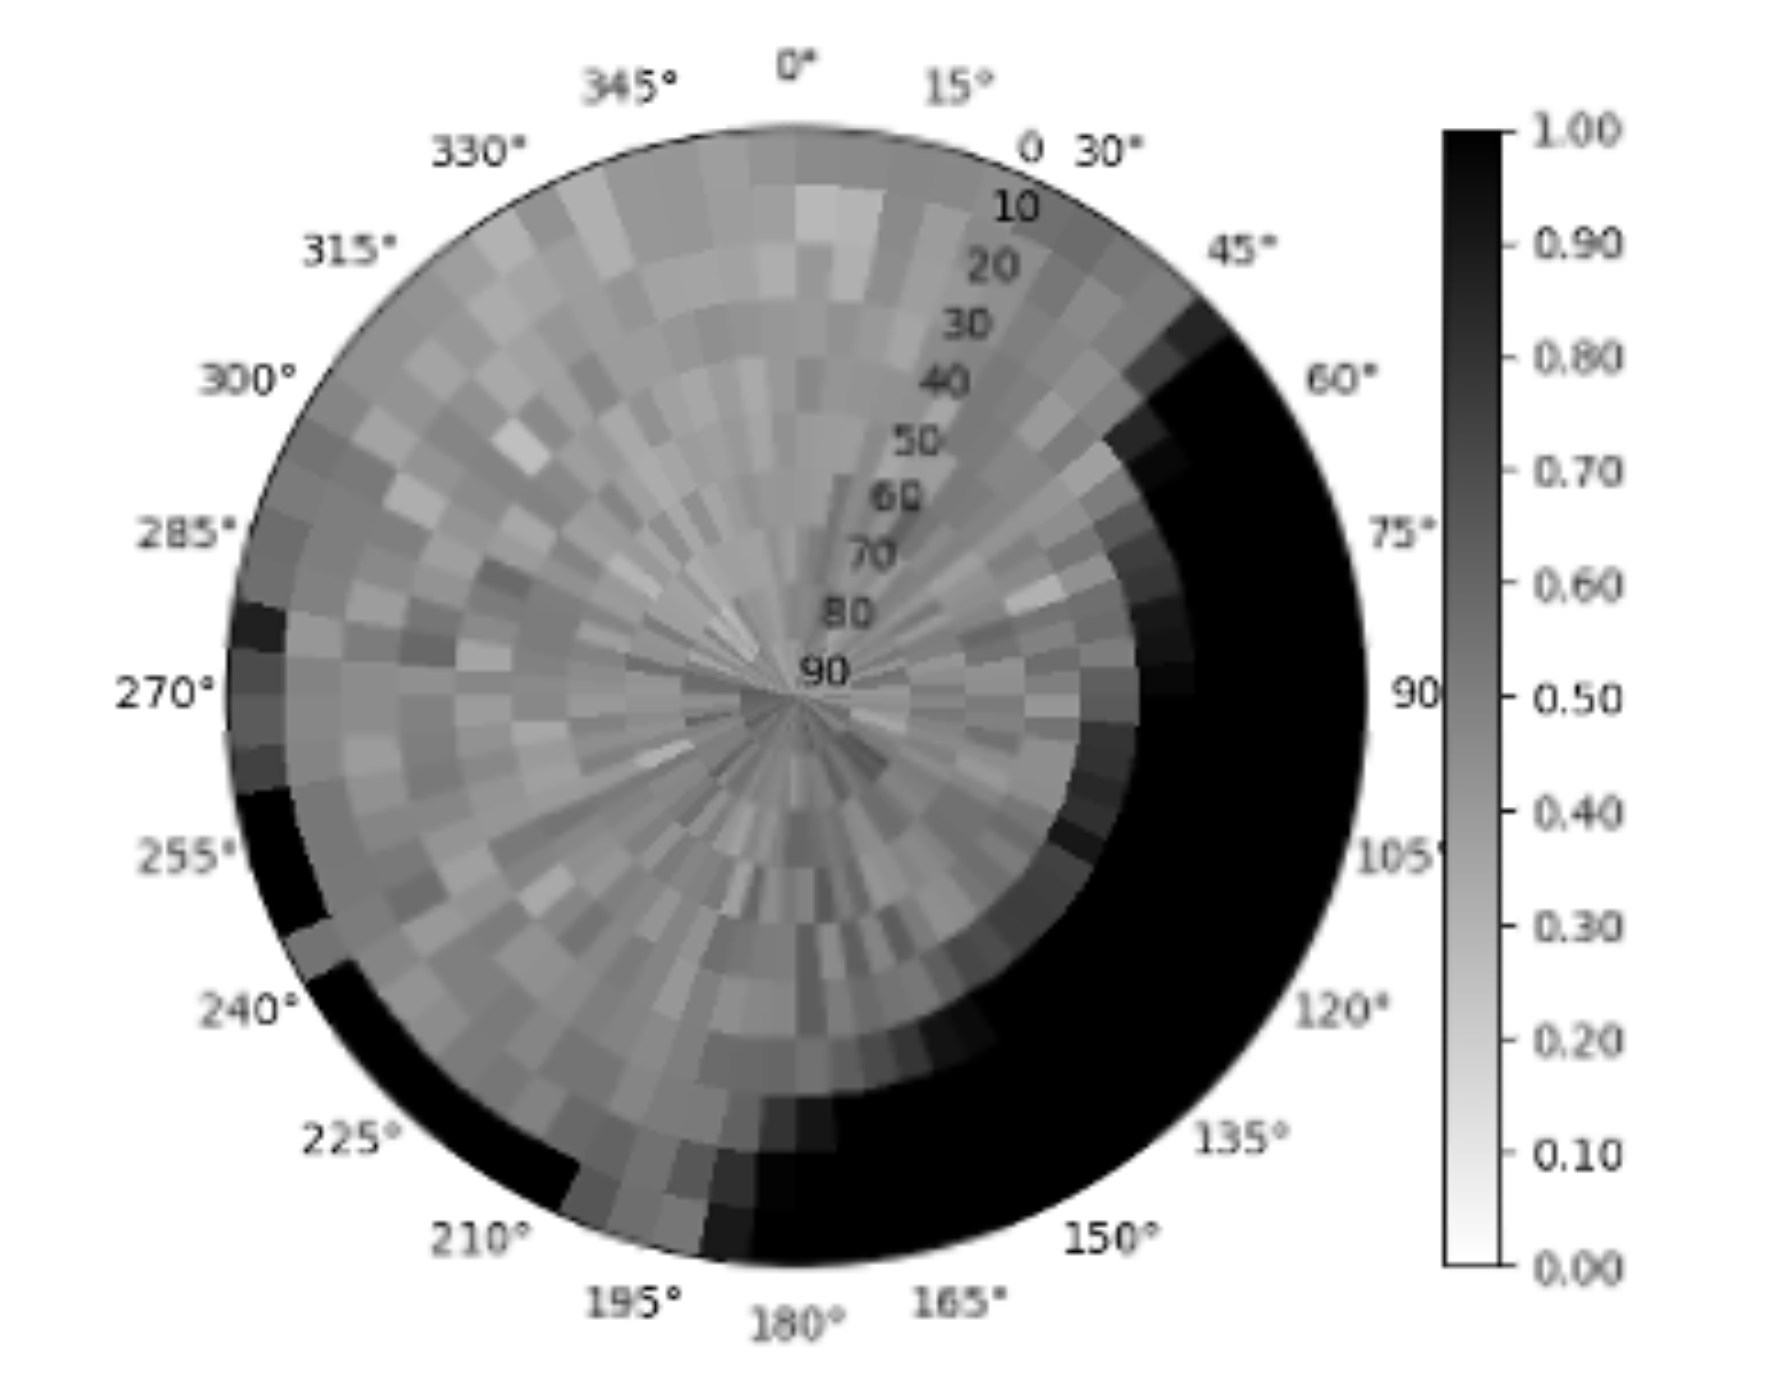
\includegraphics[width=\linewidth]{images/solar-masks-whole-building.png}
  \caption{LOD-1}
  \label{fig:sm-whole-building}
\end{subfigure}
\begin{subfigure}{.4\textwidth}
  \centering
  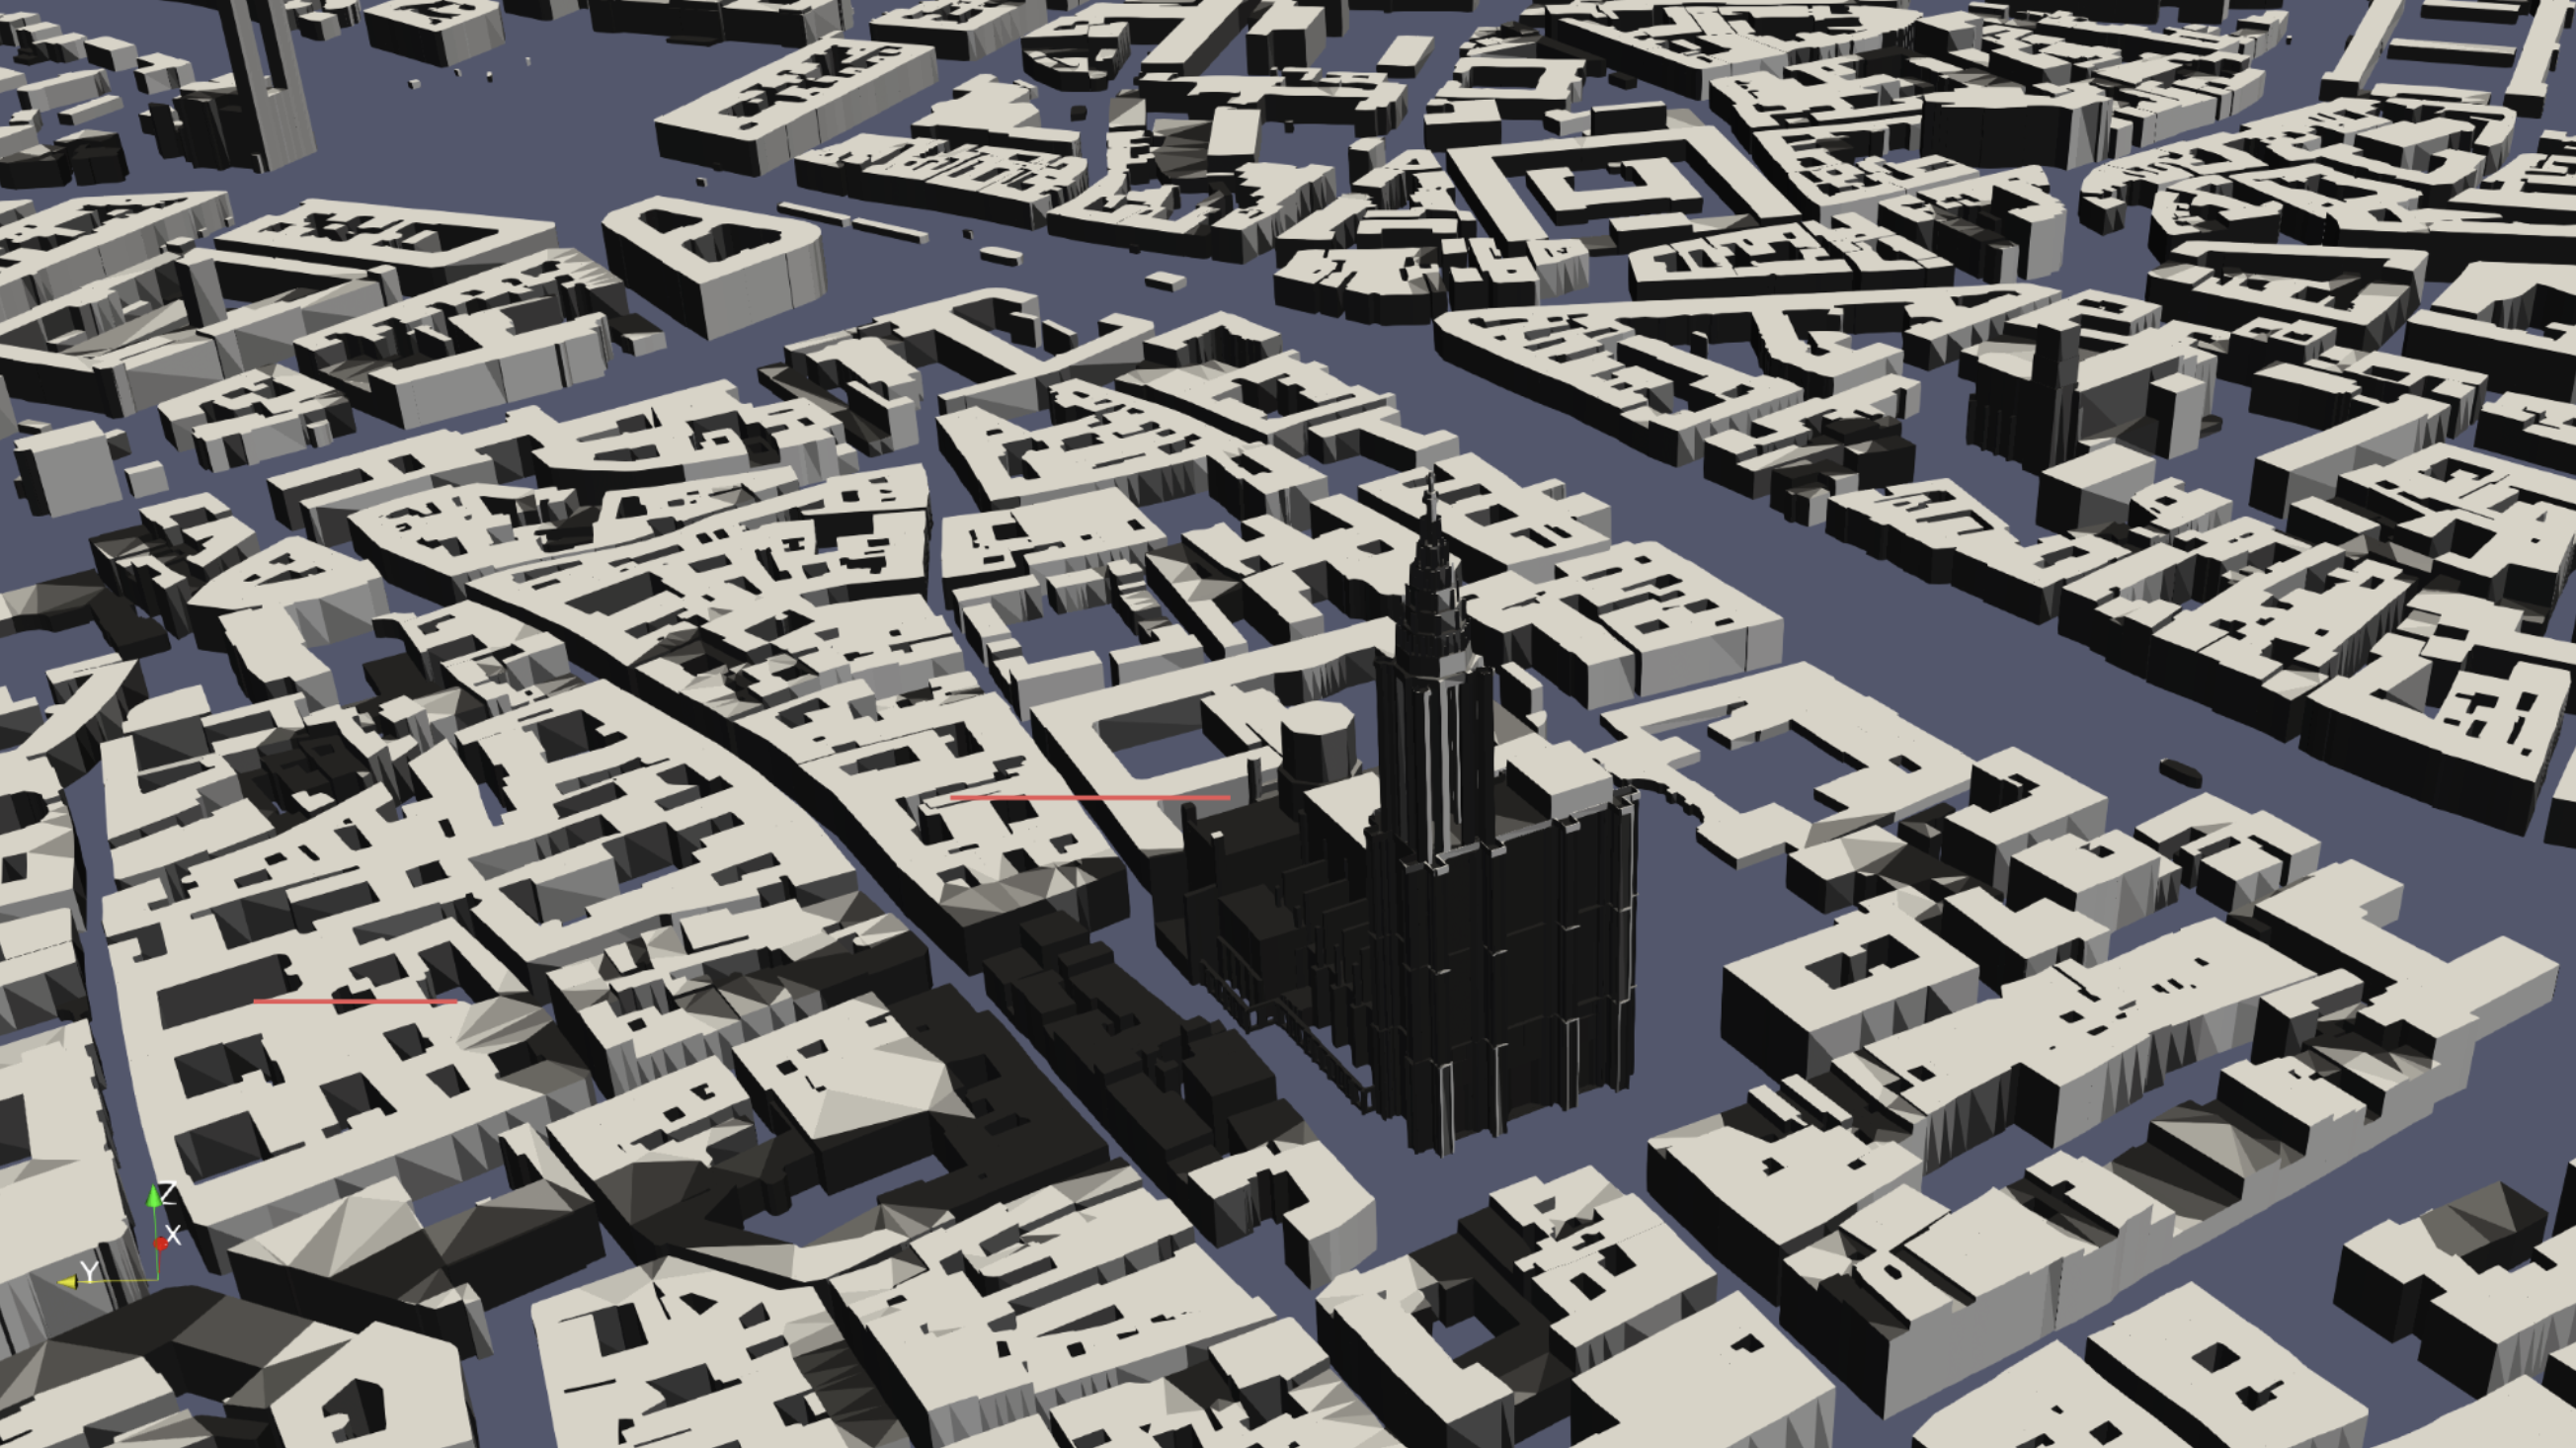
\includegraphics[width=\linewidth]{images/solar-masks-strasbourg.png}
  \caption{LOD-1 Large scale}
  \label{fig:sm-strasbourg}
\end{subfigure}
\begin{subfigure}{.4\textwidth}
  \centering
  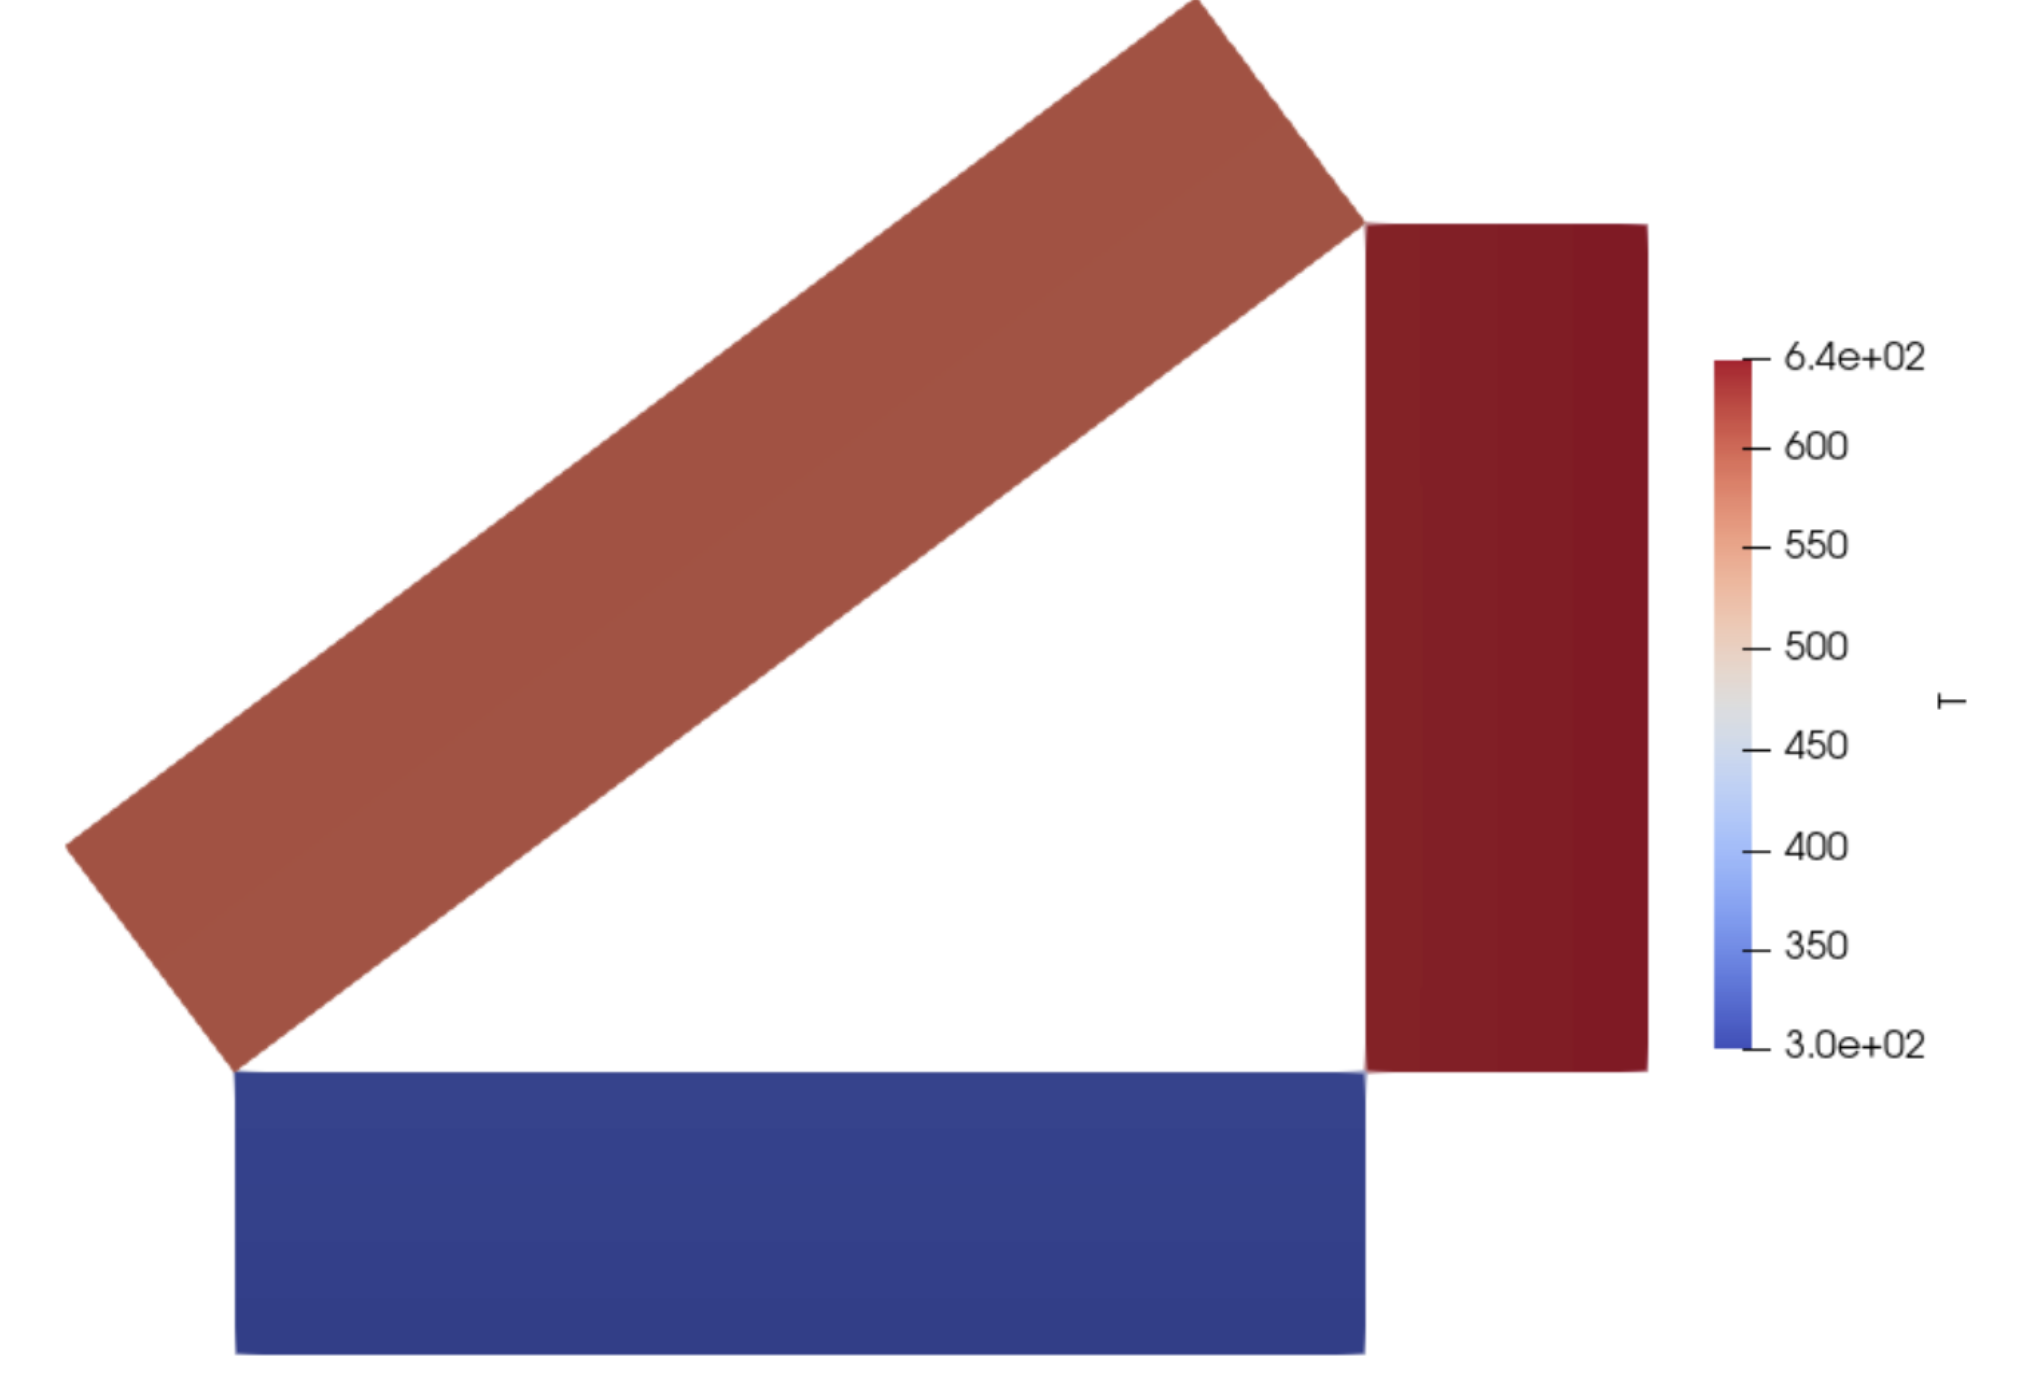
\includegraphics[width=\linewidth]{images/view-factors-benchmark.png}
  \caption{Heat transfer benchmark in 2D including view factors}
  \label{fig:view-factor}
\end{subfigure}
\caption{Solar masks and view factors computations}
\label{fig:solar-masks-vf}
\end{figure}

In the figure~\ref{fig:solar-masks-vf}, we illustrate \textit{(i)} the solar masks of building face oriented eastwise for a discretization of the sun position in the panel~\ref{fig:sm-building-east}, \textit{(ii)} the solar masks for an entire building for discretization of the sun position in the panel~\ref{fig:sm-whole-building}, \textit{(iii)} a visualization of the solar mask early morning of the city center of Strasbourg in panel~\ref{fig:sm-strasbourg} and \textit{(iv)} an image of a standard benchmark for the computation of view-factors and solving the heat transfer problems between three building blocks in 2D subsequently in panel~\ref{fig:view-factor}.

\subsubsection{Heat Transfer Modeling with Feel++ and Modelica}
In the Urban Building Energy Model (UBEM), heat transfer analysis is a crucial component for predicting energy consumption, internal air temperature variations, and overall building energy performance. This analysis is facilitated by a combination of Feel++ and Modelica, which together enable detailed simulations of heat dynamics within urban buildings.

\paragraph{Modelica for Multizone Heat Transfer}
Modelica offers extensive capabilities for multizone building energy simulations, utilizing models that range from simple (LOD-0) to more complex (LOD-1) representations. The multizone approach in Modelica is particularly useful for modular and scalable simulations, where each zone of the building can be modeled with different fidelity based on the simulation requirements. This method leverages the generation of Functional Mock-up Units (FMUs) which integrate seamlessly into larger C/C++ applications, providing a robust framework for handling complex simulations involving multiple interacting systems.

\paragraph{Finite Element Analysis with Feel++}
Complementing Modelica's capabilities, Feel++ provides robust tools for finite element analysis, particularly in handling the detailed aspects of heat transfer within urban environments. It uses advanced numerical methods like reduced basis methods for rapid scenario testing and parallel-in-time algorithms for efficient simulations. This is particularly important for assessing the impact of solar radiation and external shading, which are modeled using both geometric and dynamic shading masks derived from solar paths.

\paragraph{Integrated Approach}
The integration of Feel++ and Modelica is exemplified in their use of shading masks and view factors, critical for accurate solar heat gain calculations. These masks are computed using Monte Carlo simulations and ray tracing methods to assess the percentage of solar radiation impacting various building surfaces. This data feeds into the Modelica simulations, enhancing the accuracy of the thermal load predictions.

\paragraph{Challenges and Solutions}
One of the main challenges in urban building simulation is managing the computational load, which is addressed through hybrid computing strategies that leverage both CPUs and GPUs. This approach ensures that large-scale simulations, necessary for city-wide energy analysis, remain feasible and efficient. Additionally, the mesh partitioning techniques discussed earlier are employed to optimize the data handling and processing times, further integrating the spatial data management with the thermal modeling processes.

By utilizing the combined strengths of Feel++ for detailed finite element analysis and Modelica for system-level energy simulation, the UBEM framework is a tool capable of addressing the complex dynamics of urban heat transfer and energy management.

Continuous Integration (CI) and Continuous Deployment (CD) are pivotal in developing and operating the Urban Building pilot. These practices enable efficient management of complex simulation software, ensuring seamless integration and deployment across various computational infrastructures.

CI practices handle complex dependencies and computational requirements specific to urban building simulations. Key features include automated testing, code quality checks, and automated builds, ensuring the software remains robust and maintainable.

CD practices are tailored to manage deployment complexities across different HPC environments using containerization through Apptainer. This approach facilitates consistent, reproducible deployments, optimizing performance and resource utilization.

\section{CI/CD Framework for the Urban Building Pilot}
The Urban Building pilot utilizes the Feel++ framework, supported by a robust CI/CD framework that facilitates efficient development and deployment. This section outlines how GitHub Actions and Docker streamline the entire process, ensuring the robustness and productivity of the software development lifecycle.

\subsection{Standard CI/CD DevOps}
The development and deployment of the Urban Building pilot are enhanced through a CI/CD pipeline employing GitHub Actions and Docker. GitHub Actions automate real-time workflows to compile, test, and validate code changes, thereby facilitating rapid development cycles and ensuring code quality. Docker, on the other hand, provides a containerized environment that encapsulates Feel++ along with its dependencies, ensuring consistent operations across diverse computing environments. These Docker images, customized for various system requirements, are maintained on the GitHub Container Registry (ghcr.io) to accommodate a wide range of deployment scenarios.

\begin{figure}
    \centering
    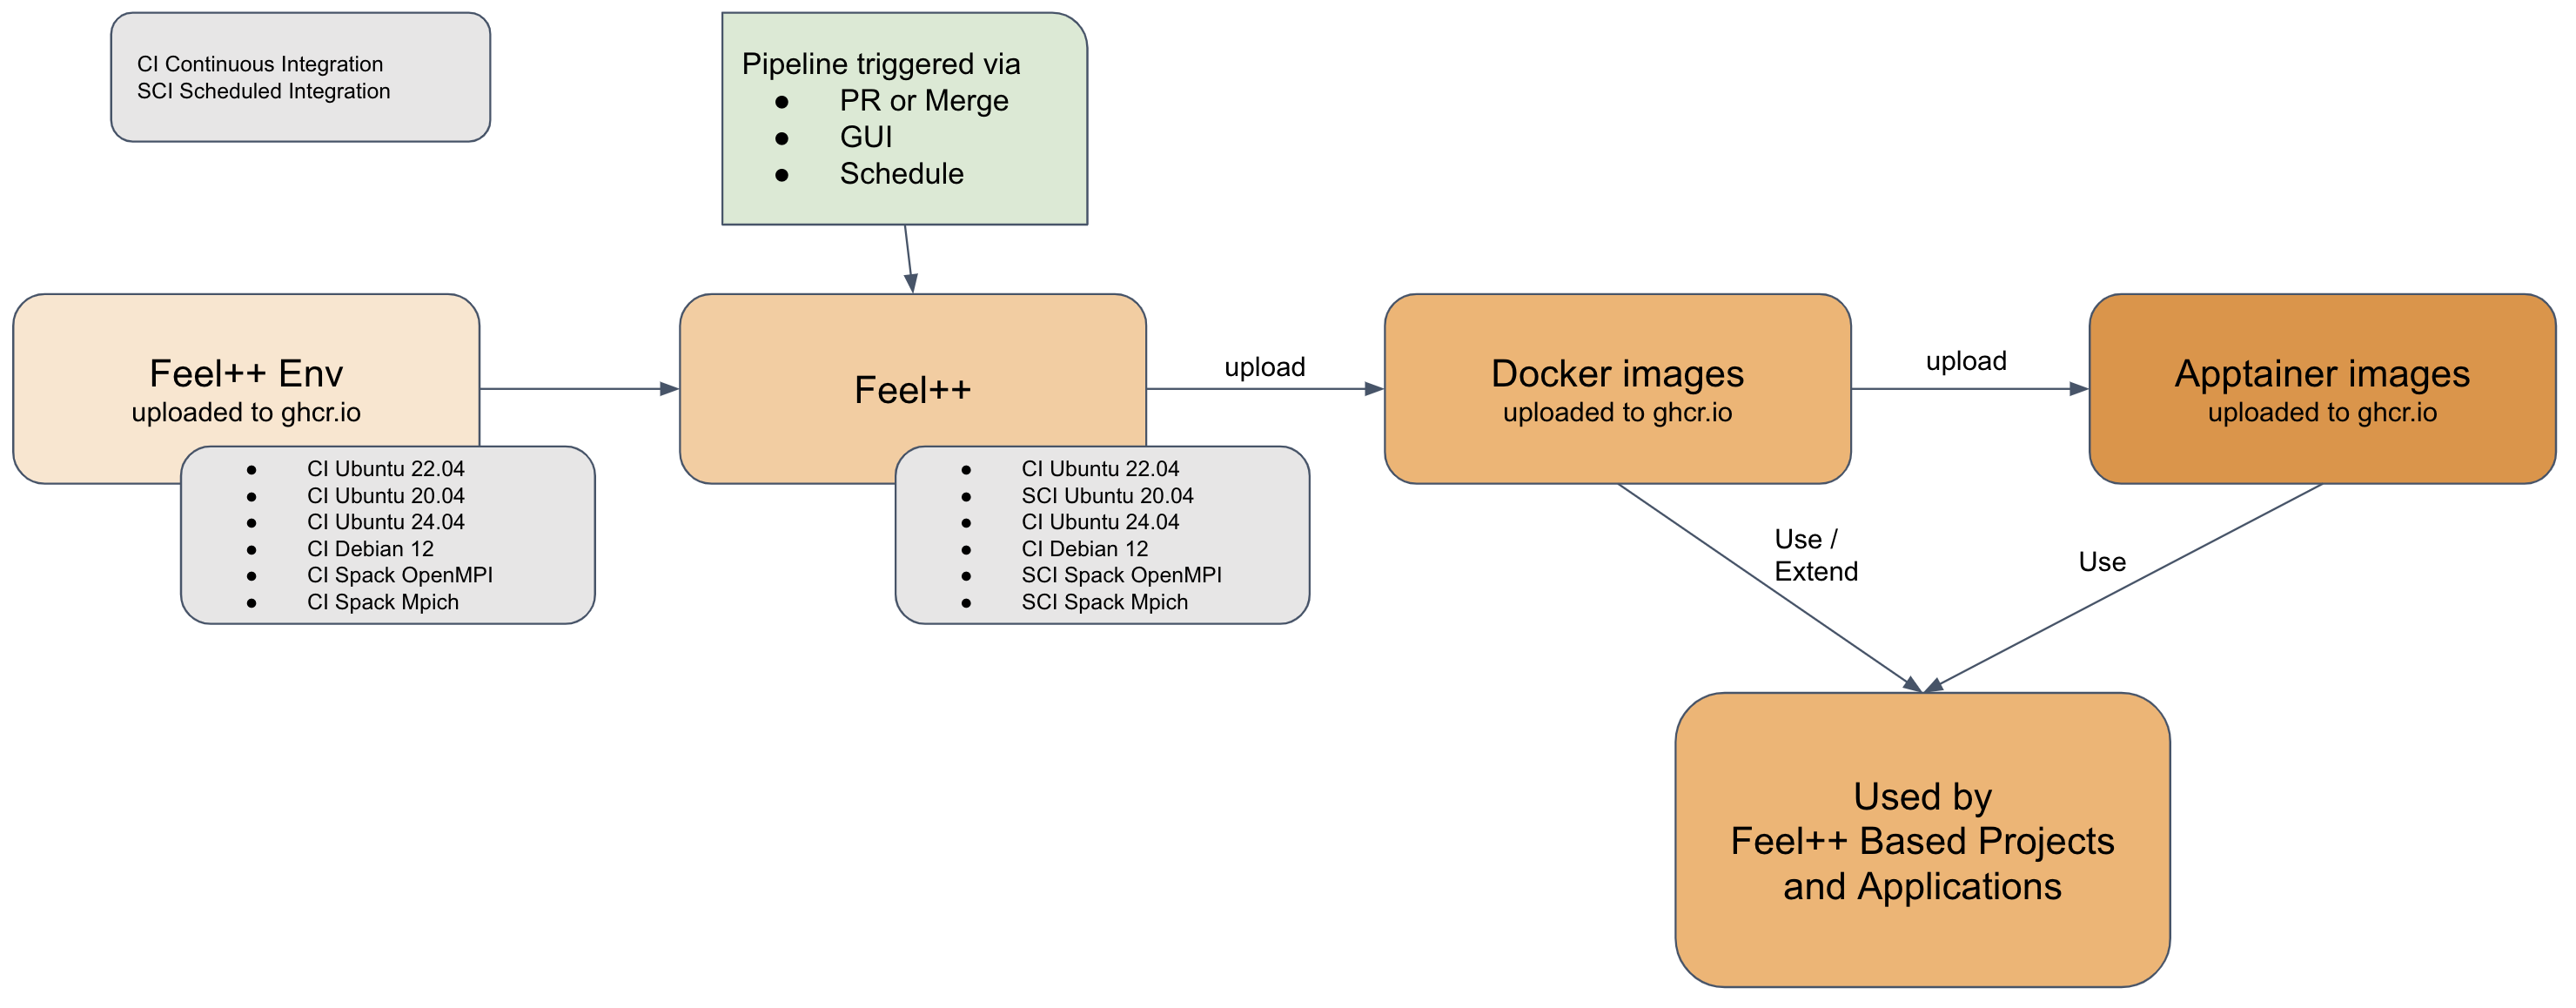
\includegraphics[width=\textwidth]{images/feelpp-devops.png}
    \caption{CI/CD devops for Feel++}
    \label{fig:feelpp-devops}
\end{figure}
This CI/CD workflow, see Figure~\ref{fig:feelpp-devops}, is crucial for efficiently integrating and deploying updates across all projects that utilize the Feel++ framework. It includes mechanisms for:
\begin{enumerate}
    \item \textbf{Pull Requests and Merges:} Triggering CI to verify that new code integrations meet all tests and standards.
    \item \textbf{Graphical User Interface (GUI):} Enabling developers to manually trigger pipelines through a GUI, which facilitates rapid deployment or testing.
    \item \textbf{Scheduled Runs:} Conducting regular updates and maintenance checks to ensure continuous system integrity and responsiveness.
\end{enumerate}

\subsection{HPC Operations (HPC-Ops)}
For high-performance computing applications, the Urban Building pilot incorporates specialized HPC-Ops practices that ensure the software performs consistently across various HPC systems. This advanced CI/CD strategy uses Apptainer (formerly Singularity) for secure and reproducible deployments across HPC environments without root privileges.

Figure~\ref{fig:feelpp-hpcops} illustrates the HPC CI/CD or HPC-ops workflow for Feel++. The Urban Building 
\begin{figure}
    \centering
    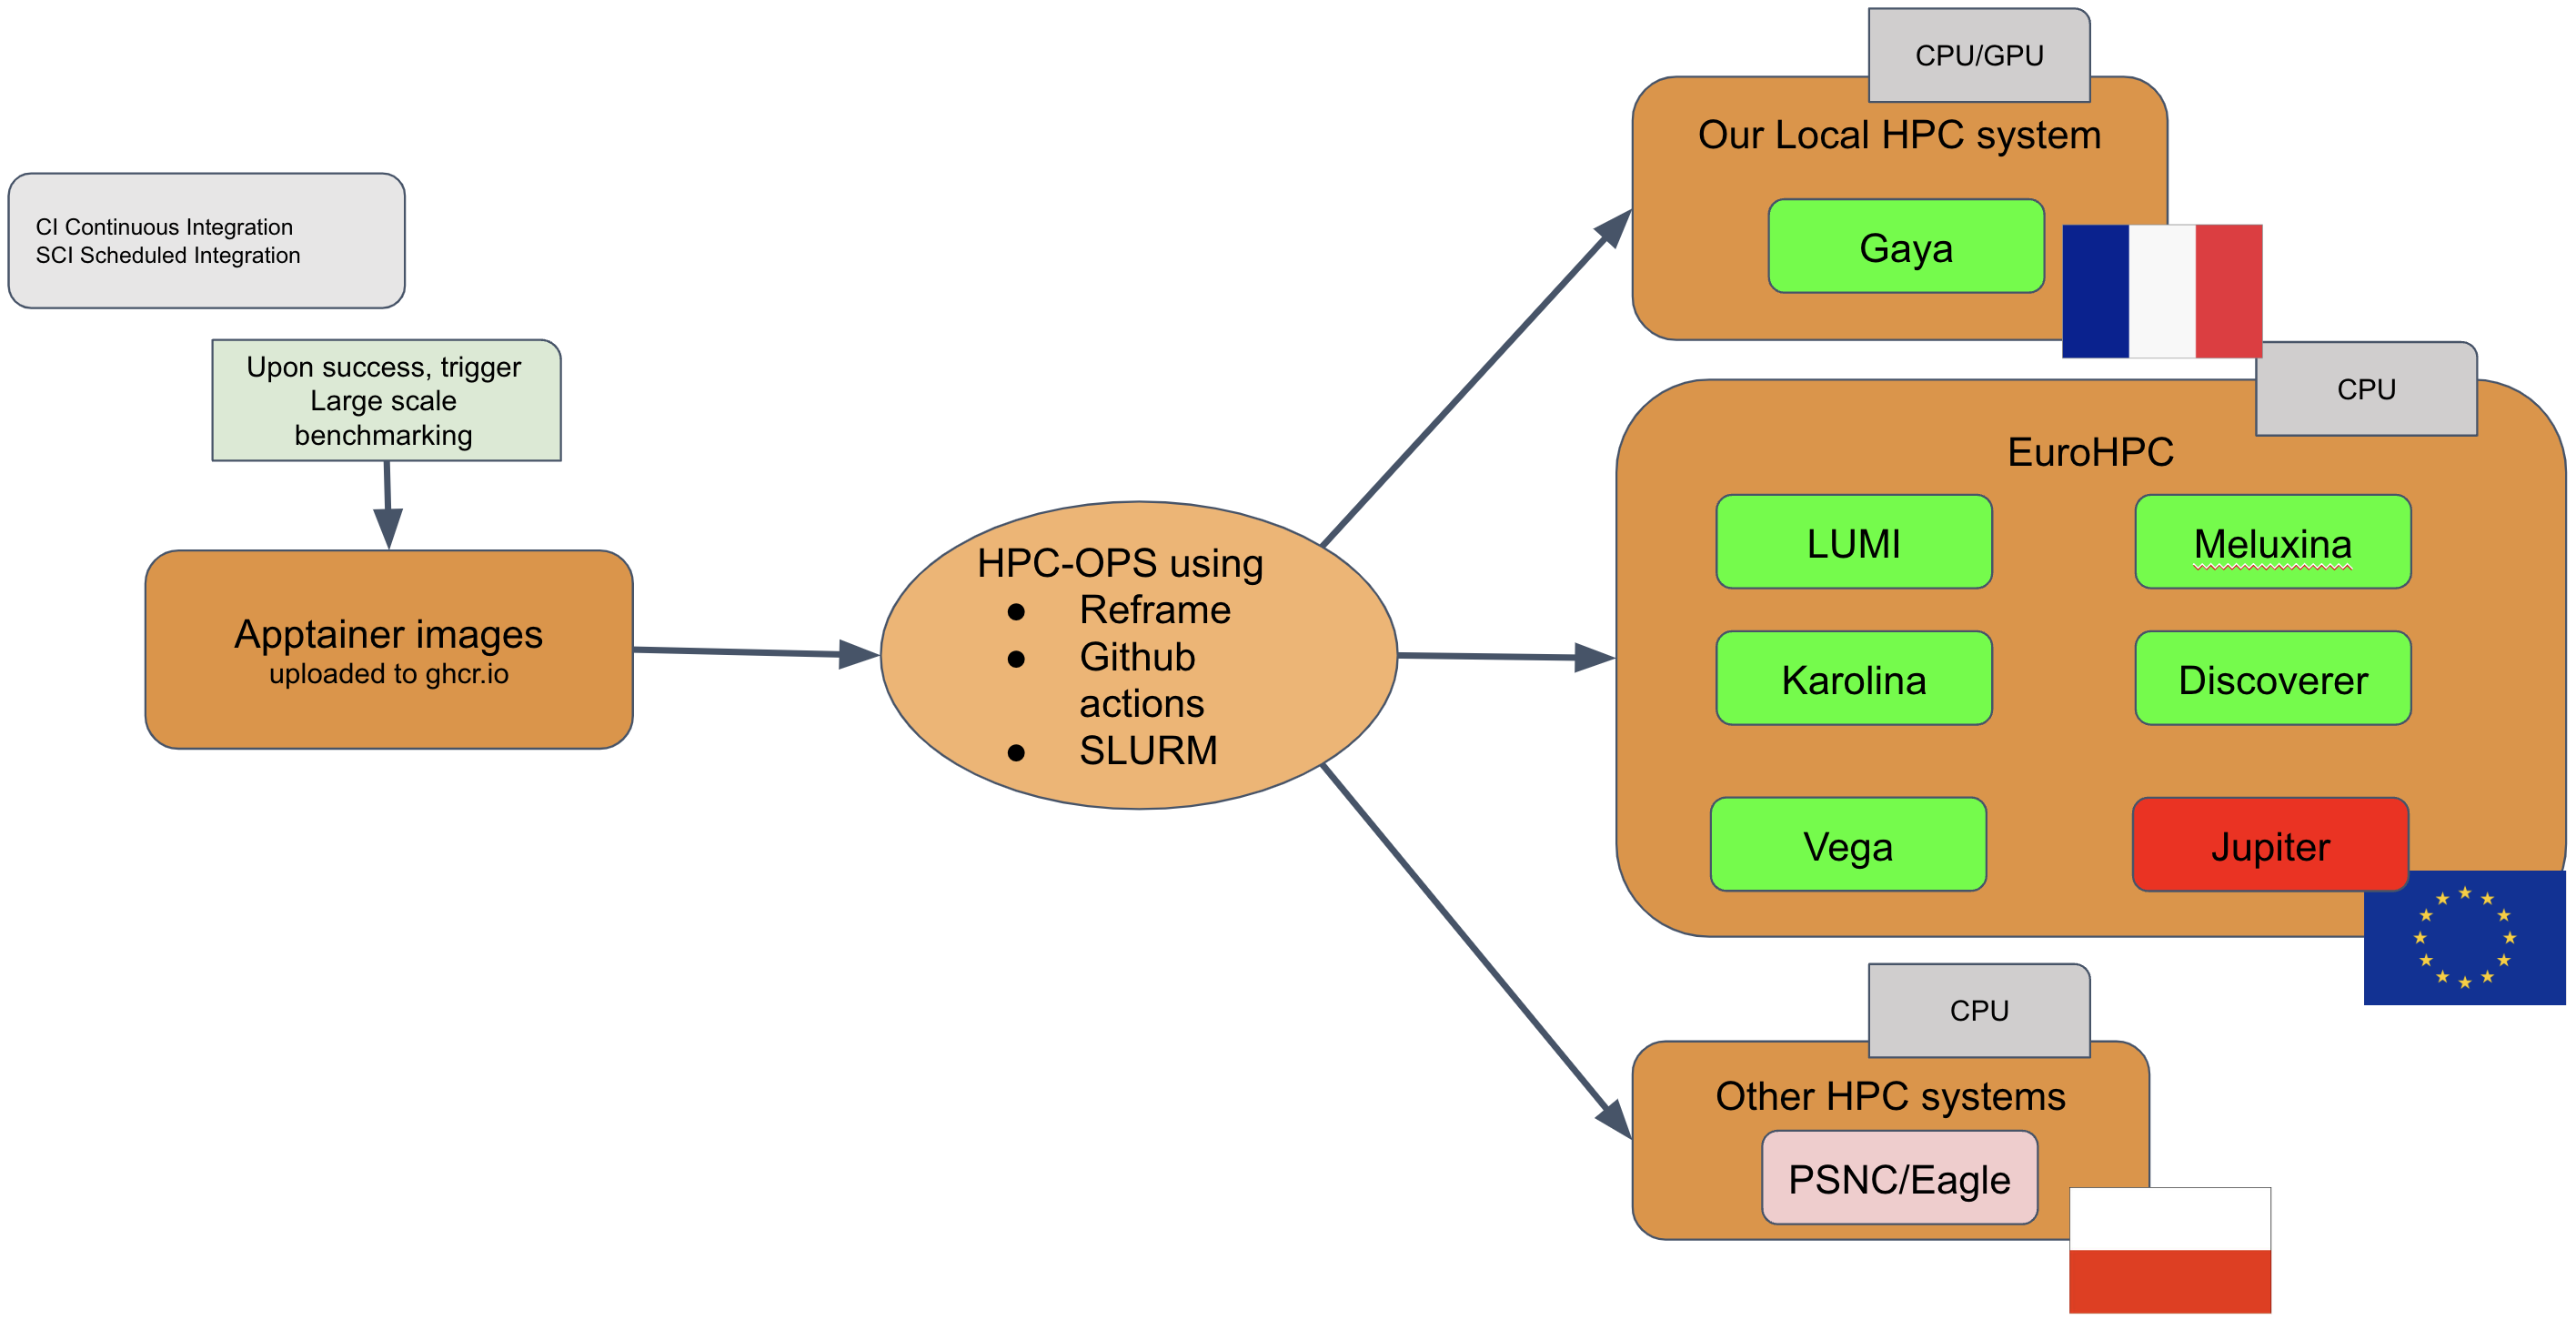
\includegraphics[width=\textwidth]{images/feelpp-hpcops.png}
    \caption{CI/CD HPC-ops for Feel++}
    \label{fig:feelpp-hpcops}
\end{figure}

The tools and Strategies for HPC-Ops are  \textit{(i) }\textbf{Reframe:} Utilized to define and manage systematic benchmarks that are reproducible across different HPC environments, facilitating the testing of performance and scalability;
\textit{(ii)}\textbf{SLURM:} Employs its REST API if available, otherwise scripted SLURM usage for CI/CD for scheduling and managing jobs on integrated HPC systems, allowing programmable job submission and monitoring directly from CI workflows; and \textit{(iii)} \textbf{Apptainer:} Ensures that Docker containers can be deployed securely and efficiently in HPC settings, supporting portability and consistency.

The integration with HPC systems such as LUMI, Karolina, Meluxina, and Discoverer, as well as local and international platforms like Gaya and PSNC's Eagle, enhances the capability to perform large-scale simulations. The operations include automatic testing that triggers larger scale tests on designated HPC nodes once new changes are integrated and verified by standard CI/CD pipelines.

\textbf{Monitoring and Reporting:}
Performance results from these operations are automatically captured and uploaded to the HiDALGO2 portal, ensuring that stakeholders have real-time access to performance reports and that decision-makers can review comprehensive data to guide further optimization and development efforts.

This comprehensive framework underlines the commitment of the HiDALGO2 project to leveraging cutting-edge computational technologies to enhance urban simulation studies, ensuring high performance and accuracy of the Urban Building models. It sets a benchmark for integrating modern software frameworks with advanced HPC infrastructures to significantly advance computational research and applications.

\begin{figure}
    \centering
    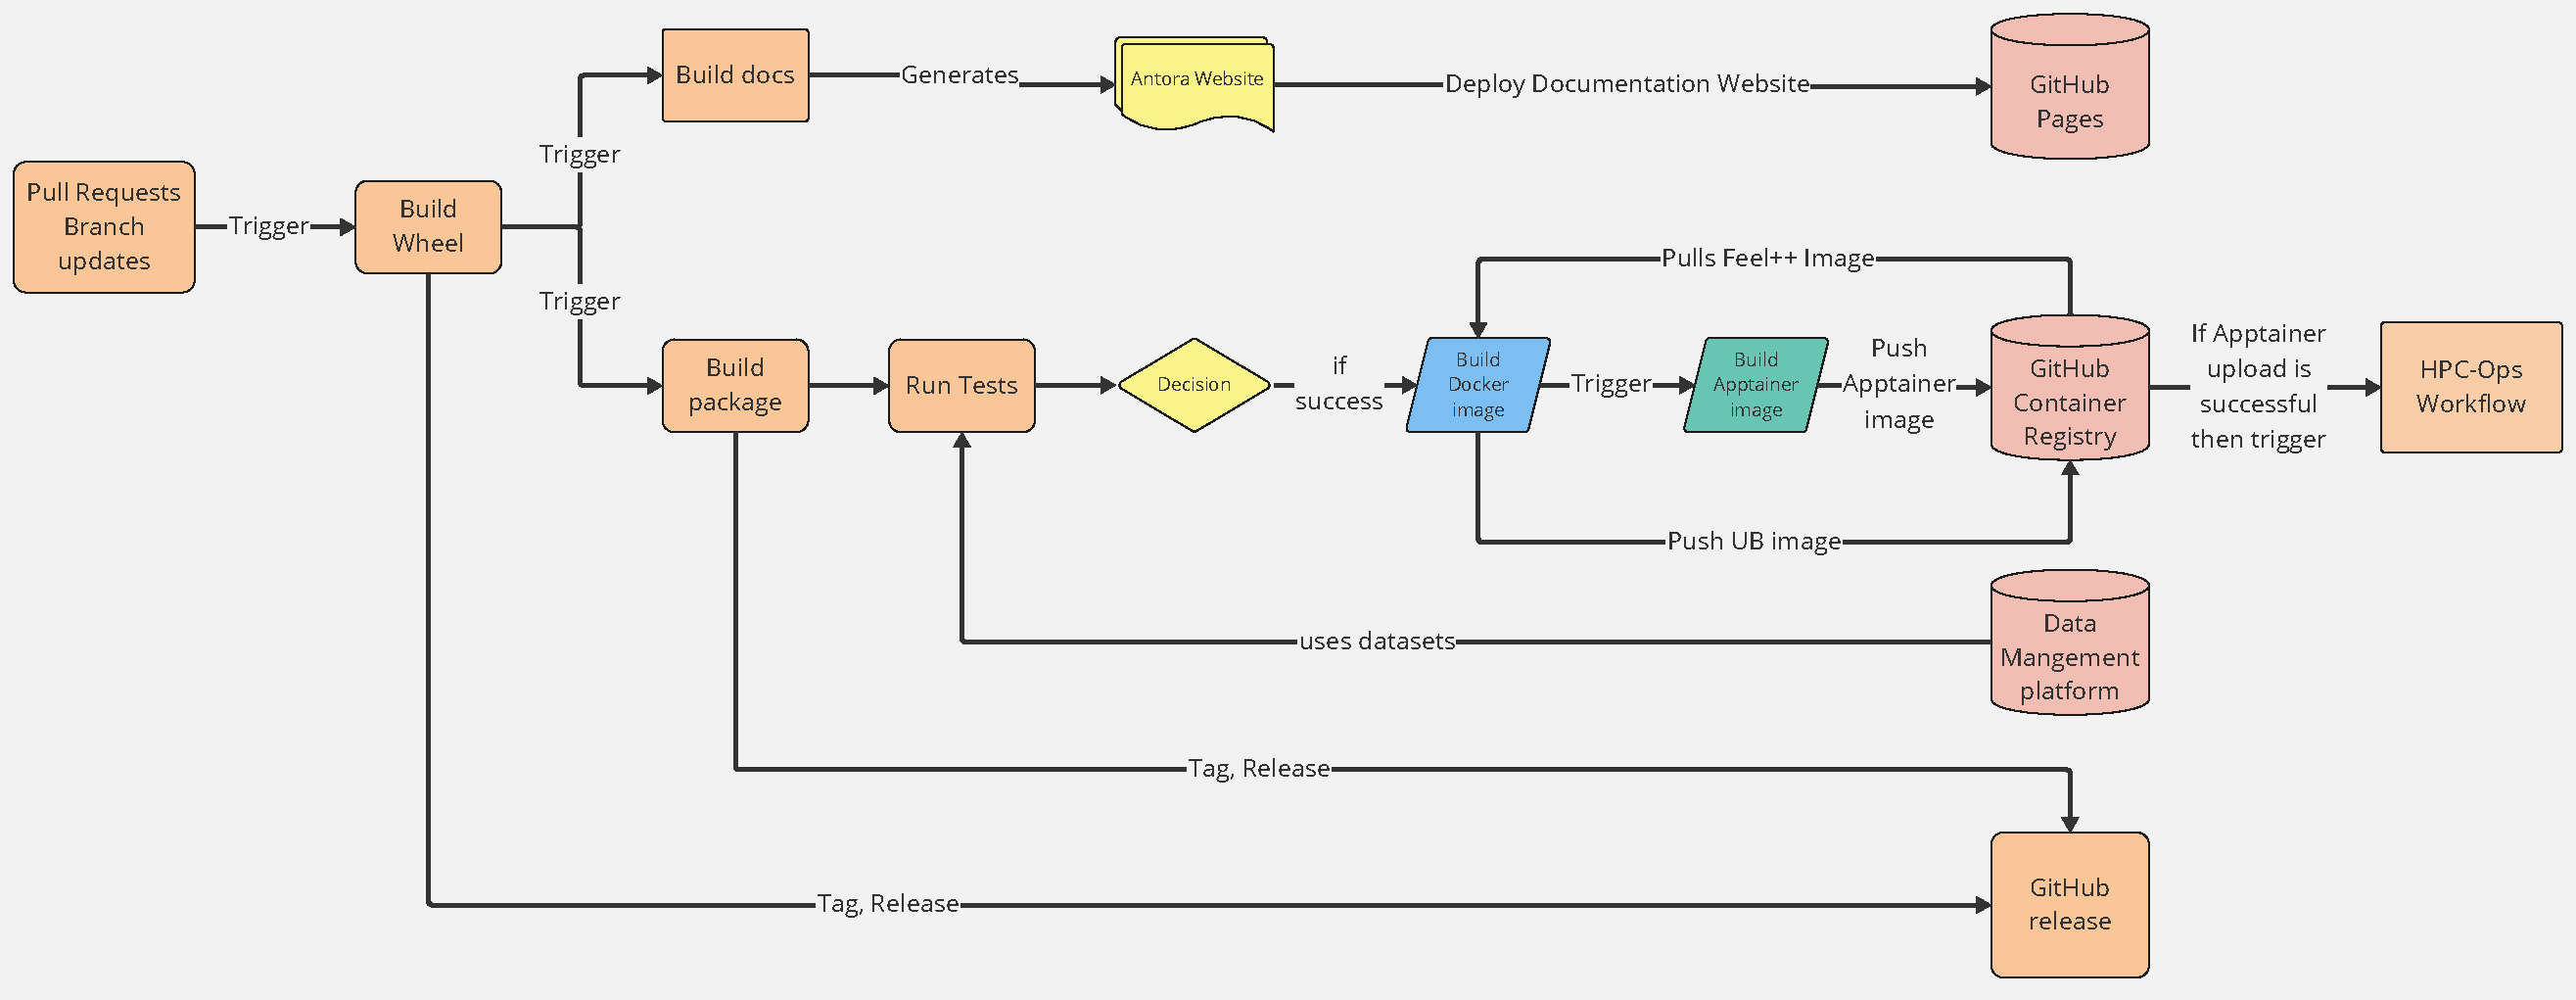
\includegraphics[width=\textwidth]{images/ub-devops.pdf}
    \caption{Urban Building standard Devops}
    \label{fig:ub-devops}
\end{figure}

\begin{figure}
    \centering
    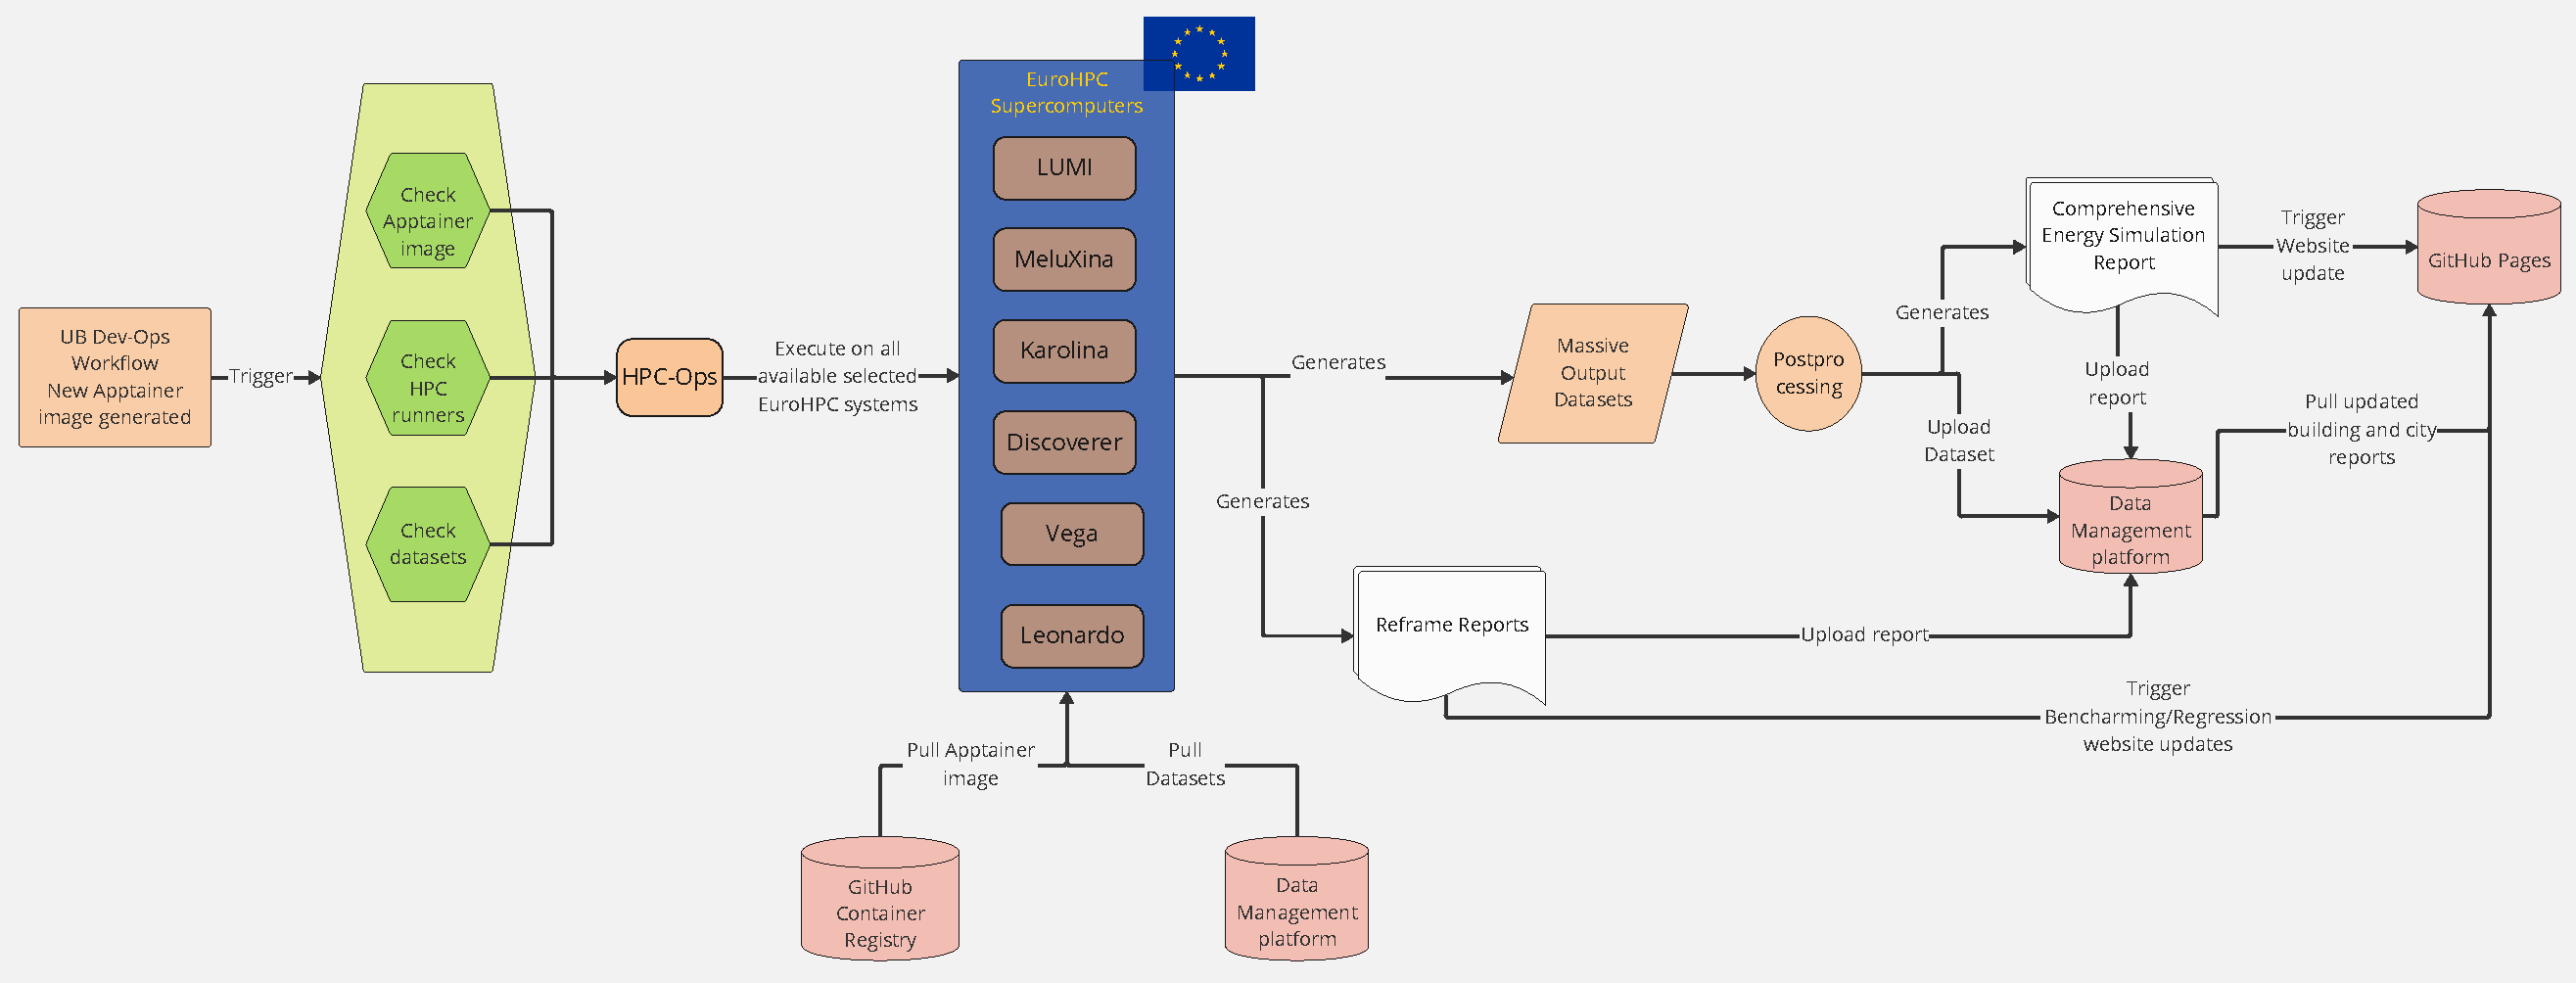
\includegraphics[width=\textwidth]{images/ub-hpcops.pdf}
    \caption{Urban Building HPC Ops workflow}
    \label{fig:ub-hpcops}
\end{figure}
\section{Conclusion}
The CI/CD practices in Feel++ not only enhance the development lifecycle of the framework itself but also ensure that all dependent projects maintain high standards of reliability, security, and performance. The integration of Docker and Apptainer into the workflow enables wide-ranging deployment scenarios from personal computing environments to high-performance computing clusters.

The integration of Feel++ within the HiDALGO2 project's Urban Building pilot through a sophisticated CI/CD framework supports the project's goal to enhance urban sustainability and air quality. The continuous development, testing, and deployment facilitated by this framework are vital for adapting to evolving urban challenges and computational needs.

CI/CD practices in HiDALGO2 are vital for advancing urban building simulations, supporting the EU's energy efficiency goals, and contributing to the reduction of greenhouse gas emissions in the urban sector.

\begin{credits}
\subsubsection{\ackname} Funded  by  the  European  Union.  This  work  has  received  funding  from  the European  High  Performance  Computing  Joint  Undertaking  (JU)  and  Poland, Germany,  Spain,  Hungary,  France,  Greece  under  grant  agreement  number: 101093457. This  publication  expresses  the  opinions  of  the  authors  and  not  necessarily those of the EuroHPC JU and Associated Countries which are not responsible for any use of the information contained in this publication

Part of this work was also funded by \textit{(i)} the France 2030 NumPEx Exa-MA (ANR-22-EXNU-0002) project managed by the French National Research Agency (ANR), \textit{(ii)} AMIES the french agency for interaction between mathematics and enterprises and \textit{(iii)} CNRS through its prematuration programme.

We acknowledge the EuroHPC Joint Undertaking for awarding this project access through  EuroHPC Development Access grants EHPC-DEV-2024D05-025 and EHPC-DEV-2023D08-047 to the EuroHPC supercomputers : \textit{(i)} Lumi, hosted by CSC (Finland) and the Lumi consortium, \textit{(ii)} Meluxina hosted by LuxProvide, Luxembourg, \textit{(iii)} Karolina hosted by IT4Innovations National Supercomputing Center, Czechia, \textit{(iv)} Discoverer osted by Sofia Tech Park, Bulgaria, \textit{(v)} Vega hosted by IZUM, Slovenia, and \textit{(vi)} Leonardo hosted by CINECA, Italy.


Finally the authors would like to acknowledge the many fruitful discussions with our partners Luc Kern from Synapse Concept and Leopold Fischer from Cisco Meraki, our colleagues \textit{(i)} from Hidalgo2 ICCS Kostis Nikas, Aristomenis Theodoridis and Petros Anastasiadis for the discussions on Reframe and joining their EuroHPC access grant, \textit{(ii)} Hidalgo2 HLRS Sameer Haroon for the discussions on CI/CD, \textit{(iii)} Pierre Alliez from INRIA Titane and Andreas Fabri from Geometry Factory regarding the discussions on CGAL and using Polygon Repair, and finally \textit{(iv)} our former colleague Zohra Djatouti, now at Kipsum, which whom we initiated this endeavor. 

% \subsubsection{\discintname}
% It is now necessary to declare any competing interests or to specifically
% state that the authors have no competing interests. Please place the
% statement with a bold run-in heading in small font size beneath the
% (optional) acknowledgments\footnote{If EquinOCS, our proceedings submission
% system, is used, then the disclaimer can be provided directly in the system.},
% for example: The authors have no competing interests to declare that are
% relevant to the content of this article. Or: Author A has received research
% grants from Company W. Author B has received a speaker honorarium from
% Company X and owns stock in Company Y. Author C is a member of committee Z.
\end{credits}

\bibliographystyle{splncs04}
\bibliography{references}

\end{document}